\documentclass[twocolumn, 11pt, letterpaper]{article}

% Font
\usepackage[utf8]{inputenc}
\usepackage{MinionPro} 
\input{glyphtounicode}
\pdfgentounicode=1 
\usepackage{microtype}

% Format
\usepackage[letterpaper, margin = 1in]{geometry}
\setlength{\columnsep}{18pt}
\setcounter{secnumdepth}{0}
\usepackage[compact]{titlesec}
\titleformat*{\section}{\centering\normalfont\Large\bfseries}
\titleformat*{\subsection}{\raggedright\normalfont\normalsize\bfseries}
\titleformat*{\subsubsection}{\raggedright\normalfont\normalsize\bfseries\itshape}
\usepackage{authblk}
\renewcommand\Affilfont{\small}
\newcommand{\refsection}{\section{References}}
\providecommand{\tightlist}{\setlength{\itemsep}{0pt}\setlength{\parskip}{0pt}}

% Links
\usepackage[colorlinks = true, linkcolor = black, urlcolor = black, citecolor = black]{hyperref} 

% Figures
\usepackage{graphicx}
\usepackage[labelfont = bf, font = small, labelsep = newline, singlelinecheck = false]{caption}

% Tables
\usepackage{booktabs}
\usepackage{tabularx}

% References
\newenvironment{CSLReferences}[2]{}{}

% Frontmatter
\title{ Double Standards in Judging Collective Action\thanks{} }
\author[1]{Nils K. Reimer}
\affil[1]{University of California, Santa Barbara, United States}
\author[2]{Marija Brankovi\'{c}}
\affil[2]{Singidunum University, Serbia}
\author[3]{Iniobong Essien}
\affil[3]{Leuphana University of L\"{u}neburg, Germany}
\author[4]{Jin X. Goh}
\affil[4]{Colby College, United States}
\author[5]{S\'{e}bastien Goudeau}
\affil[5]{University of Poitiers, France}
\author[6]{N\'{o}ra A. Lantos}
\affil[6]{E\"{o}tv\"{o}s Lor\'{o}nd University, Hungary}
\author[7]{Jenny Veldman}
\affil[7]{KU Leuven, Belgium}


\date{July 15, 2022}

\begin{document}

\twocolumn[
  \begin{@twocolumnfalse}
    \maketitle
    \begin{abstract}
      \noindent Collective action is a powerful force driving social
change but often sparks contention about what actions are acceptable
means to effect social change. In four studies (total \emph{N} = 2,246),
we investigated double standards in judging collective action---that is,
whether observers will judge the same protest actions as more acceptable
if the protesters are ingroup members and their cause aligns with the
ingroup's interests (\emph{identity-based double standards}) or if the
protesters' cause aligns with the observers' ideological positions
(\emph{ideology-based double standards}). In two studies, we developed
an instrument of 25 controversial protest actions, based in item
response theory, to measure where people draw the line between
acceptable and unacceptable forms of collective action. In two
preregistered experiments, we used this instrument to test for double
standards in judging collective action for workers' rights in the United
Kingdom and for or against defunding the police in the United States. We
found evidence for ideology-based, but not for identity-based, double
standards: Participants judged the same protest actions to be more
acceptable when the protesters' cause aligned with their own
(system-challenging) ideological position---but showed no ingroup bias
when judging collective action by ingroup and outgroup members. Our
findings have theoretical and practical implications for understanding
the often divided response to prominent social movements.
    \end{abstract}
  \end{@twocolumnfalse}
  % \renewcommand{\abstractname}{Statement of Relevance}
  % \begin{@twocolumnfalse}
  %   \maketitle
  %   \begin{abstract}
  %   \noindent 
  %   \end{abstract}
  % \end{@twocolumnfalse}
]

{
  \renewcommand{\thefootnote}%
    {\fnsymbol{footnote}}
  \footnotetext[1]{M.B.--J.V. are listed in alphabetical order. This research was supported by a Seedcorn Research Grant from the European Association of Social Psychology.}
}

\noindent Protest movements often spark contention about what actions
are acceptable means of protest. Reactions to Black American athletes
kneeling during the national anthem to protest racist police violence
are a case in point. Kneeling during the national anthem is not violent,
disruptive, or illegal. And yet, only 29\% of White Americans (66\% of
Black Americans) and 11\% of Republicans (59\% of Democrats) considered
it appropriate for Black athletes to protest in this way (YouGov, 2017).
Indeed, Black athletes who had participated in the protests faced a
backlash in public opinion (Lacina, 2020). This and other examples
suggest that \emph{who} the protesters are and \emph{what} they are
protesting influences how acceptable observers judge their actions to
be.

In this paper, we examine double standards in judging collective
action---that is, whether observers judge the same protest actions as
more or less acceptable depending on their own and the protesters' group
memberships (\emph{identity-based double standards}) or on the
protesters' cause and how it aligns with their own ideological positions
(\emph{ideology-based double standards}). In two studies, we first
develop an instrument of 25 controversial protest actions, based in item
response theory, to capture double standards in judging collective
action. In two preregistered experiments, we then use this instrument to
test for double standards in judging protest actions for workers' rights
in the United Kingdom and for or against defunding the police in the
United States. We find evidence for ideology-based, but not for
identity-based, double standards: People judge the same protest actions
to be more acceptable when the protesters' cause aligns with their own
(system-challenging) ideological positions---but do not show ingroup
bias when judging collective action by ingroup and outgroup members.

\hypertarget{double-standards-in-judging-collective-action}{%
\subsection{Double Standards in Judging Collective
Action}\label{double-standards-in-judging-collective-action}}

Collective action---that is, any action taken by group members to
advance a shared political goal (for similar definitions, see Becker,
2012; van Zomeren, 2016)---is a powerful force driving social change.
For example, Black Lives Matter protests lastingly shifted public
discourse about racial inequity toward antiracist ideas (Dunivin et al.,
2022).

Collective action can take many forms. Psychologists distinguish between
\emph{normative} collective action that seeks to achieve a political
goal while conforming to the norms of the existing social system and
\emph{non-normative} collective action that violates those norms (Wright
et al., 1990). Recent research has shown that this distinction matters
for how people respond to collective action. Shuman et al. (2021) showed
that non-normative, non-violent collective action is more effective than
either normative or violent collective action at gaining concessions
from those most resistant to social change. Feinberg et al. (2020)
demonstrated, however, that observers are less supportive of social
movements that use extreme protest actions. Similarly, Teixeira et al.
(2020) found that advantaged-group members perceive non-normative
collective action by disadvantaged-group members as more damaging to
their ingroup's social image and are thus less supportive of such
action. Verkuyten et al. (2022) found that, in general, the public tends
to be intolerant of non-normative collective action. This means that
activists face the dilemma that non-normative collective action might be
most effective at gaining concessions but that it also risks reducing
popular support for a cause. Together, these studies show that the
distinction between normative and non-normative collective action is
psychologically and societally consequential.

Research has, for the most part, relied on ad-hoc distinctions between
what researchers themselves considered normative and non-normative
collective action. In liberal democracies, researchers tend to consider
actions such as signing petitions, voting in elections, or peaceful
protest to be normative and actions such as blocking traffic, damaging
property, or violent protest to be non-normative. But, as the examples
in the first paragraph show, the distinction between normative and
non-normative collective action might instead be in the eye of the
beholder.

In this research, we move this distinction from the researcher's
intuition into the realm of scientific investigation and test for double
standards in where people draw the line between acceptable and
unacceptable forms of collective action. For that purpose, we define a
double standard as judging the same action as more or less acceptable
depending on who is performing the action and for what reason (for an
analogous definition, see Foschi, 2000).\footnote{Feinberg et al. (2020)
  provided incidental evidence for double standards in judging
  collective action as, in a manipulation check, Black participants
  rated Black Lives Matter protests as less extreme than White
  participants and liberal participants rated protest actions for
  progressive causes as less extreme than conservative participants.} In
this section, we derive predictions from social psychological theories
about how identity-based and ideology-based double standards could lead
people to judge the same protest actions as more or less acceptable
depending on who the protesters are and what they are protesting.

\hypertarget{identity-based-double-standards}{%
\subsubsection{Identity-Based Double
Standards}\label{identity-based-double-standards}}

Social Identity Theory (Tajfel \& Turner, 1979; for a recent review, see
Reimer et al., 2022) argues that just as people show self-serving biases
to achieve positive self-esteem, they show ingroup-serving biases to
achieve positive social identities. In other words, they think about
ingroup and outgroup in ``me''--``not me'' terms and favor ingroup
members (``us'') over outgroup members (``not us,'' Brewer, 2007).

One domain in which ingroup bias manifests is judgements about other
people's actions. Hewstone (1990) reviewed research showing that people
make ingroup-serving causal attributions when judging actions by ingroup
and outgroup members, for example, by attributing negative behavior by
outgroup members to internal causes but attributing negative behavior by
ingroup members to external causes. Valdesolo \& DeSteno (2007)
demonstrated that participants judged the same selfish action as less
unfair when performed by themselves or an ingroup member than when
performed by an outgroup member. Other studies (Abrams et al., 2013;
Endevelt et al., 2021; for exceptions, see Mendoza et al., 2014; Pinto
et al., 2010) provided further evidence for ingroup bias in judging
moral transgressions by ingroup and outgroup members.

In the same vain, we propose that ingroup bias results in identity-based
double standards in judging collective action by ingroup and outgroup
members. That is, we hypothesize that people will judge the same protest
actions as more acceptable if the protesters are ingroup members
(\emph{Hypothesis 1a}) or if the cause of the protest aligns with the
ingroup's interests (\emph{Hypothesis 1b}). This hypothesis could
explain why, for example, far more Black than White Americans considered
it appropriate for Black athletes to kneel down to protest police
violence against Black Americans (YouGov, 2017). Notably, this
hypothesis applies equally to historically disadvantaged groups
mobilizing against social injustice and to historically advantaged
groups defending their group's position.

\hypertarget{ideology-based-double-standards}{%
\subsubsection{Ideology-Based Double
Standards}\label{ideology-based-double-standards}}

System Justification Theory (Jost \& Banaji, 1994; for a recent review,
see Jost, 2020) argues that people are motivated to defend, justify, and
bolster the prevailing social, economic, and political system because
doing so serves basic epistemic, existential, and relational needs. Both
advantaged and disadvantaged groups are thought to be motivated to
justify the existing system, although the strength of this motivation
and its expression vary across individuals and situations.

While system justification often leads people to resist social change,
its relationship to collective action depends on the goal of the action.
Jost et al. (2017) argued that research on collective action needs to
distinguish between system-challenging protest aimed at changing an
unequal status quo and system-supporting protest aimed at maintaining or
defending an unequal status quo. Osborne et al. (2019) showed that, for
members of both advantaged and disadvantaged groups, system
justification is associated with supporting system-supporting actions
but with opposing system-challenging actions.

Just as system justification shapes support for, and opposition to,
collective action, we propose that it results in ideology-based double
standards in what actions people consider acceptable forms of collective
action. First, we hypothesize that people will judge the same protest
actions as more acceptable if the protest supports, rather than
challenges, the system (\emph{Hypothesis 2a}). This hypothesis reflects
the assumption that the motivation to justify the system is, to some
extent, universal. Second, we hypothesize that people will judge the
same protest actions as more acceptable if they endorse
system-justifying beliefs and the protest supports the system or if they
reject system-justifying beliefs and the protest challenges the system
(\emph{Hypothesis 2b}). Notably, this hypothesis implies a symmetry in
how people with different ideological orientations judge
system-supporting and system-challenging collective action.

As system-justifying beliefs are closely related to political
conservatism (Jost et al., 2003), this hypothesis could explain partisan
differences in what actions liberals and conservatives consider
acceptable means of protest for progressive and conservative causes.
Ideology-based double standards could, for example, explain why far more
Democrats than Republicans considered it appropriate to kneel during the
national anthem to protest racist police violence (YouGov, 2017).

\hypertarget{using-item-response-theory-to-detect-double-standards}{%
\subsection{Using Item Response Theory to Detect Double
Standards}\label{using-item-response-theory-to-detect-double-standards}}

\begin{figure}
\centering
\caption{Item response curves for three hypothetical protest actions}
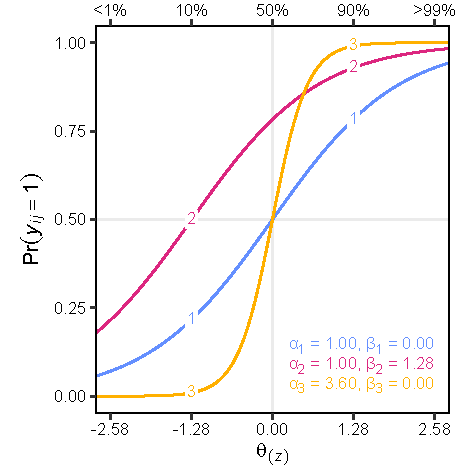
\includegraphics[scale=1]{../Scale Development/figures/figure-1}
\caption*{\textit{Note.} $\theta_{(z)}$ follows a standard normal distribution and is shown as both $z$-scores (bottom) and percentiles (top).}
\label{fig:f1}
\end{figure}

Item response theory is a a conceptual and statistical framework for
understanding how the characteristics of both items and respondents
shape responses to a set of items (DeMars, 2010). When respondents judge
whether each of a set of actions is an acceptable means of protest (1 =
\emph{yes}, 0 = \emph{no}), a two parameter logistic item response
theory model estimates responses as a function of several latent
(unobserved) parameters:
\[ \Pr ( y_{ij} = 1 ) = \text{logit}^{-1} ( \alpha_i ( \theta_j + \beta_i ) ) \]
where \(\Pr ( y_{ij} = 1 )\) is the probability that respondent \(j\)
considers action \(i\) an acceptable means of protest, \(\theta_j\)
estimates how \emph{accepting} respondent \(j\) is of various protest
actions, \(\beta_i\) estimates how \emph{acceptable} action \(i\) is,
and \(\alpha_i\) estimates how \emph{discriminating} action \(i\) is.

Figure \ref{fig:f1} illustrates those relationships for three
hypothetical protest actions. \(\theta_{(z)}\) is the
\emph{z}-standardized tendency for a participant to be more accepting of
various actions so that \(\beta_i\) determines the probability that the
average respondent (\(\theta_{(z)} = 0\)) considers an action an
acceptable means of protest. Action 2 (\(\beta_2 = 1.28\)) is more
acceptable than Actions 1 and 2 (\(\{ \beta_2, \beta_3 \} = 0\)) as the
average respondent is more likely to consider the former (\(\Pr = .78\))
than the latter (\(\Pr = .50\)) acceptable means of protest. Action 3
(\(\alpha_3 = 3.60\)) is more discriminating than Actions 1 and 2
(\(\{ \alpha_1, \alpha_2 \} = 1\)) as the slope for the relationship
between how accepting a respondent is and how likely they are to
consider an action acceptable is steeper for the former action. This
means that knowing whether someone considers Action 3 acceptable
provides more information about them than knowing whether they consider
Actions 1 or 2 acceptable.

In this research, item response theory serves two purposes. First, item
response theory provides a statistical framework for scale development.
In Studies 1 and 2, we select the most discriminating and informative
actions to build an instrument for capturing double standards in the
experiments. Second, item response theory provides a formal and
statistical definition of double standards in judging collective action
as respondents being more accepting of the same protest actions
depending on who the protesters and what they are protesting. In
Experiments 1 and 2, we operationalize double standards as the
differences in \(\theta_{(z)}\) between conditions which, as
\(\theta_{(z)}\) is \(z\)-standardized, correspond to Cohen's \(d\)
effect sizes.

\hypertarget{purpose-of-the-present-research}{%
\subsection{Purpose of the Present
Research}\label{purpose-of-the-present-research}}

The first purpose of our research is to develop an instrument to measure
where people draw the line between acceptable and unacceptable forms of
collective action. In Study 1, we ask participants to generate more and
less extreme protest actions and compile a pool of protest actions for
scale development. In Study 2, we ask participants to rate how
acceptable they consider each of those protest action to be and use item
response theory to select the most discriminating and informative
protest actions for our instrument. In so doing, we build an instrument
that enables both present and future research to capture double
standards in judging collective action. In this way, our research
situates the distinction between normative and non-normative collective
action in the eye of the beholders and opens it to scientific
investigation.

The second purpose of our research is to test for double standards in
judging collective action---that is, whether people judge the same
protest actions as more acceptable if the protesters' are ingroup
members or the protesters' cause aligns with the ingroup's interests
(\emph{Hypothesis 1a}, \emph{1b}) or if the protesters' cause aligns
with their own system-justifying or system-challenging motives
(\emph{Hypotheses 2a}, \emph{2b}). In Experiment 1, we use the
instrument developed in Studies 1 and 2 to test for double standards in
how acceptable participants consider collective action for workers'
rights in the United Kingdom. By varying both the participants' and the
protesters' group memberships (working/middle class), Experiment 1
compares the relative evidence for identity-based (\emph{Hypothesis 1a},
\emph{1b}) and ideology-based double standards (\emph{Hypothesis 2a}).
Extending Experiment 1, Experiment 2 considers both system-challenging
and system-defending collective action in the context of the 2020 Black
Lives Matter protests in the United States. By varying the protesters'
cause (for/against defunding the police) as well as the participants'
and the protesters' group memberships (Black/White), Experiment 2
compares the relative evidence identity-based (\emph{Hypothesis 1a},
\emph{1b}) and ideology-based double standards (\emph{Hypothesis 2a},
\emph{2b}). Together, the preregistered experiments provide a
comprehensive test of the hypothesized double standards in judging
collective action.

\hypertarget{scale-development}{%
\section{Scale Development}\label{scale-development}}

In two studies, we developed an instrument of 25 protest actions to
capture double standards in judging collective action.

\begin{figure*}[!t]
\centering
\caption{Examples of protest actions rated in Study 2}
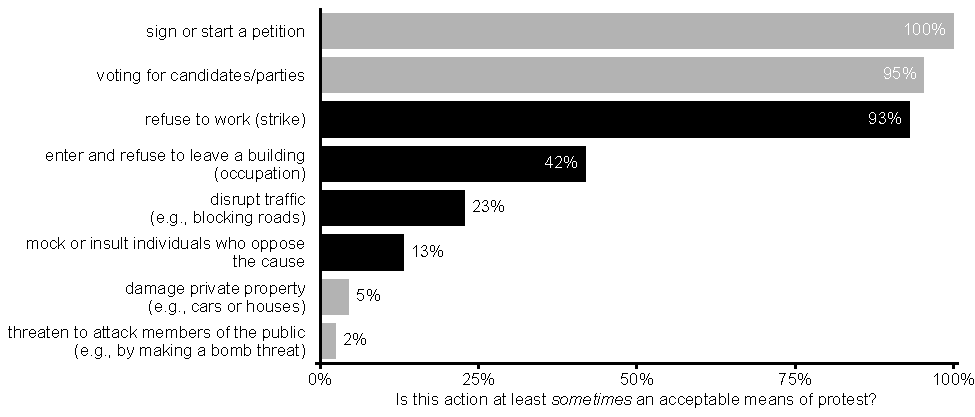
\includegraphics[scale=1]{../Scale Development/figures/figure-2}
\caption*{\textit{Note.} Percentages reflect the proportion of participants who thought that an action was \textit{sometimes}, \textit{often}, or \textit{always} an acceptable means to a advance a cause. Darker bars mark actions that were included in the final scale.}
\label{fig:f2}
\end{figure*}

\hypertarget{study-1}{%
\subsection{Study 1}\label{study-1}}

In Study 1, we compiled protest actions from participants' responses and
other sources. We recruited 60 participants from the Prolific subject
pool, all of whom were citizens of the UK or the US. To increase the
socioeconomic diversity of our sample, we recruited 30 non-students
without a university degree, 15 non-students with a university degree,
and 15 current university students.

Participants first read an accessible definition of what a social group
is and that collective action is any action group members take to
promote the interests of their social group. Participants were then
asked to name between five and ten actions that fit that definition.
Participants were encouraged to think of actions that varied in how
acceptable they were in their opinion. We recoded responses into a
smaller set of unique actions, which we supplemented with protest
actions from the psychological and political science literature (e.g.,
Sharp, 1973). This process resulted in 72 actions that varied in how
acceptable we would expect them to be. For details, see Supplemental
Online Material (SOM).

\hypertarget{study-2}{%
\subsection{Study 2}\label{study-2}}

In Study 2, we measured how acceptable participants judged the actions
from Study 1 to be and applied item response theory to develop an
instrument to capture double standards in judging collective action. We
recruited 158 participants (\(\textit{Mdn} = 30\) years, age range:
18--68 years; 103 women, 52 men, 2 other, 1 prefer not to say) from the
Prolific subject pool, all of whom were citizens of the UK or the US. To
increase the socioeconomic diversity of our sample, we recruited 80
non-students without a university degree, 37 non-students with a
university degree, and 41 current university students. We excluded 15
participants who failed an attention check, leaving a final sample of
143 participants for our analyses.

Participants again read an accessible definition of collective action.
Participants were then asked to think of different causes and
circumstances and to rate how often a given action would be an
acceptable means for a group to advance one of these causes (1 =
\emph{never}, 2 = \emph{rarely}, 3 = \emph{sometimes}, 4 = \emph{often},
5 = \emph{always}). In addition, participants rated how disruptive,
violent, and extreme they considered an action to be (1 = \emph{not at
all}, 4 = \emph{very}) and how positive or negative they felt, in
general, about an action (1 = \emph{very positive}, 5 = \emph{very
negative}). Each participant rated 20 of the 72 actions from Study 1 so
that each action was rated by 29--53 participants.

We estimated a graded response model (Bürkner, 2021; Samejima,
1997)---an item response theory model for ordinal response
variables---for participants' ratings of how often an action would be an
acceptable form of collective action.\footnote{Ratings of how often a
  given action would be an acceptable form of collective action were
  strongly and negatively correlated with how disruptive, violent, and
  extreme participants considered the action to be and how negative they
  felt about it (Table S3).} Based on the results, we selected the 25
most discriminating, informative, and relevant protest actions to form
an instrument for measuring double standards in judging collective
action in Experiments 1 and 2. We selected controversial, and thus
diagnostic, actions (e.g., disrupting traffic) over actions that almost
all respondents considered acceptable (e.g., signing petitions) or
unacceptable (e.g., political violence; Figure \ref{fig:f2}). For
detailed ratings and results, see SOM.

\hypertarget{experiment-1}{%
\section{Experiment 1}\label{experiment-1}}

In Experiment 1, we used the newly developed instrument to test for
double standards in judging collective action for workers' rights in the
United Kingdom. That is, we tested whether people with either
working-class or professional jobs applied different standards when
judging collective action taken by people with either working-class or
middle-class jobs to protest against a fictitious government bill
threatening their rights.

By varying the participants' and the protesters' group memberships, we
tested the preregistered hypothesis that, in line with \emph{Hypothesis
1a} and \emph{1b}, participants would judge the same protest actions as
more acceptable if the protesters were ingroup members protesting for
the ingroup's rights than if they were outgroup members protesting for
the outgroup's rights. By comparing reactions to working-class and
middle-class protesters, we tested how observers judge collective action
by lower-status (i.e.~working-class) and higher-status (middle-class)
group members. Assuming that collective action by lower-status group
members is seen as more threatening to the unequal status quo than
collective action by higher-status group members and that people are, to
same extent, motivated to justify the system, we tested the
preregistered hypothesis that, in line with \emph{Hypothesis 2a},
participants would judge the same protest actions as more acceptable if
the protesters were from a higher-status group than if they were from a
lower-status group. In non-preregistered analyses, we further explored
whether, in line with \emph{Hypothesis 2b}, participants would judge the
same protest actions as more or less acceptable depending on their own
ideological positions. In this way, Experiment 1 provided a first test
of the hypothesized identity- and ideology-based double standards in
judging collective action.

\hypertarget{method}{%
\subsection{Method}\label{method}}

We preregistered the sample size as well as all hypotheses,
inclusion/exclusion criteria, measures, and manipulations
(\url{https://osf.io/24wrx/?view_only=8560eb60286149498f8da48bc9f9d99b}).
We made all materials, data, and analysis scripts available online
(\url{https://osf.io/d3yev/?view_only=40782034017c40f0bcecb1cc87760b62}).
We followed sample size recommendations for item response theory models
(DeMars, 2010, p. 36), planning to recruit 500 participants.

\hypertarget{study-design}{%
\subsubsection{Study Design}\label{study-design}}

We used a 2 (quasi-experimental: higher-status/lower-status
participants) \(\times\) 2 (experimental: higher-status/lower-status
protesters) between-subjects design to test our hypotheses.

\hypertarget{participants}{%
\subsubsection{Participants}\label{participants}}

We recruited 515 participants from the Prolific subject pool who were UK
citizens, 25 years old or older, and not current students.\footnote{We
  had preregistered a sample of 500 participants, before exclusions, but
  included another 15 participants who completed the study without
  returning an approval code to the Prolific platform. Participants
  received, on average, \pounds 9.00 (\$10.93) per hour of
  participation.} As preregistered, we excluded 71 participants who
failed an attention check. This resulted in a final sample of 443
participants (\(\textit{Mdn} = 41\) years, age range: 25--76 years; 272
women, 171 men, 1 non-binary). Of these, 210 participants considered
their past, current, or future jobs to be working-class jobs.
Participants in this lower-status group did not have a university degree
and placed themselves on the bottom three ranks of the subjective
socioeconomic status ladder. Another 233 participants considered their
past, current job, or future jobs to be middle-class/professional jobs.
Participants in this higher-status group had at least an undergraduate
degree and placed themselves on the top four ranks of the subjective
socioeconomic status ladder.

\hypertarget{procedure}{%
\subsubsection{Procedure}\label{procedure}}

We used a screening survey to recruit participants who satisfied our
preregistered inclusion criteria for the lower-status and higher-status
groups. For the lower-status group, we recruited 475 participants who
did not have a university degree and placed themselves on the bottom
three ranks of a subjective socioeconomic status ladder. For the
higher-status group, we recruited 400 participants who had at least an
undergraduate degree and placed themselves on the top four ranks of the
subjective socioeconomic status ladder.

In the screening survey, participants read an accessible definition of
what working-class and middle-class/professional jobs are (for details,
see SOM). Participants then answered, among other questions, whether
they considered their current job---or the jobs they had had in the past
or expected to have in the future---to be a working-class job or a
middle-class/professional job. As preregistered, we excluded
participants from the lower-status group who did not respond
``working-class job'' and participants from the higher-status group who
did not respond ``middle-class/professional job''.

We recruited 500 participants from the remaining 687 participants, 250
from the lower-status group and 250 from the higher-status group.
Participants were randomly assigned to read a vignette about a
government bill affecting either people in working-class jobs
(lower-status protesters) or people in professional jobs (higher-status
protesters). Participants in both conditions were instructed to
carefully read the vignette and to try to imagine what it would be like
if this situation was real. Participants in the lower-status protesters
condition read the following introduction:

\begin{quote}
The government, though not necessarily the current government, is going
to introduce a bill that will mostly affect people in working-class
jobs. Working-class jobs, in this case, are jobs done by skilled,
semi-skilled, unskilled manual workers or by casual workers. These are
jobs that do not usually require a university degree. Other jobs are
unlikely to be affected.
\end{quote}

\noindent Participants in the higher-status protesters condition instead
read the following introduction:

\begin{quote}
The government, though not necessarily the current government, is going
to introduce a bill that will mostly affect people in professional jobs.
Professional jobs are administrative, managerial, or other jobs that
usually require a university degree. Other jobs are unlikely to be
affected.
\end{quote}

\noindent Participants in both conditions then read an almost
identically worded paragraph:

\begin{quote}
This government measure would make it easier for companies to hire
workers during economic growth and to lay off workers during an economic
crisis. As a consequence, companies would be able to fire employees with
little notice and without giving a reason. Trade unions are opposed to
the measure. They argue that the bill would compromise job security, and
prevent employees from challenging harassment or other abuse without the
fear of being fired. People in {[}working-class/professional{]} jobs are
particularly at risk, and there is a rise in tension and outrage among
them.
\end{quote}

On the next pages, participants completed all remaining measures. On the
final page, we asked participants to recall who the people most affected
by the fictitious government bill were. As preregistered, we excluded
all participants whose response did not qualitatively match their
experimental condition.

\hypertarget{measures}{%
\subsubsection{Measures}\label{measures}}

We measured the outcome variable by asking participants to decide, for
each of 25 protest actions presented in a randomized order, whether they
thought this action was ``an acceptable means for people in
{[}working-class/professional{]} jobs to protest against the government
bill'' (1 = \emph{yes}, 0 = \emph{no}; see Table A1).

We assessed reactions to the vignette by asking participants how
outraged they would be if the government were to introduce this bill in
real life, to what extent it would affect them personally, and to what
extent the it would affect people like them (1 = \emph{not at all}, 7 =
\emph{very much}). We also asked participants to what extent they
identified with people with the kinds of jobs most affected by the
proposed bill (1 = \emph{not at all}, 7 = \emph{very much}) and how
often, if at all, they had participated in protest actions such as the
ones we asked about (1 = \emph{never}, 5 = \emph{very often}).

We measured social dominance orientation with the eight-item
\(\text{SDO}_{7(s)}\) scale (Ho et al., 2015), for example, ``it is
unjust to try to make groups equal'' (1 = \emph{strongly oppose}, 7 =
\emph{strongly favour}; McDonald's \(\omega = .89\)). A confirmatory
factor analysis model in which all items loaded onto a single factor
showed acceptable fit,
\(\chi^2 (20) = 108.69; \text{CFI} = 0.92; \text{TLI} = 0.88; \text{RMSEA} = 0.11, [0.09, 0.14]\).

We measured system-justifying beliefs with eight items (adapted from Kay
\& Jost, 2003), for example, ``in general, I find society to be fair''
(1 = \emph{strongly disagree}, 7 = \emph{strongly agree}; McDonald's
\(\omega = .89\)). A confirmatory factor analysis model in which all
items loaded onto a single factor showed acceptable fit,
\(\chi^2 (20) = 77.37; \text{CFI} = 0.94; \text{TLI} = 0.92; \text{RMSEA} = 0.09, [0.07, 0.12]\).

In the screening survey, we recorded participants' gender, age,
nationality, student status, and employment status. We also included two
three-item scales measuring social identification with people in
working-class and middle-class/professional jobs (adapted from Becker et
al., 2011) and a one-item semantic differential scale measuring
political orientation (``People often describe their political
orientation as left-wing or right-wing. On a scale from left to right,
where would you position yourself?''; 1 = \emph{left}, 7 =
\emph{right}).

\hypertarget{results}{%
\subsection{Results}\label{results}}

\begin{figure*}[!t]
\centering
\caption{Results from the preregistered (\textbf{A}) and non-preregistered (\textbf{B}) analyses for Experiment 1}
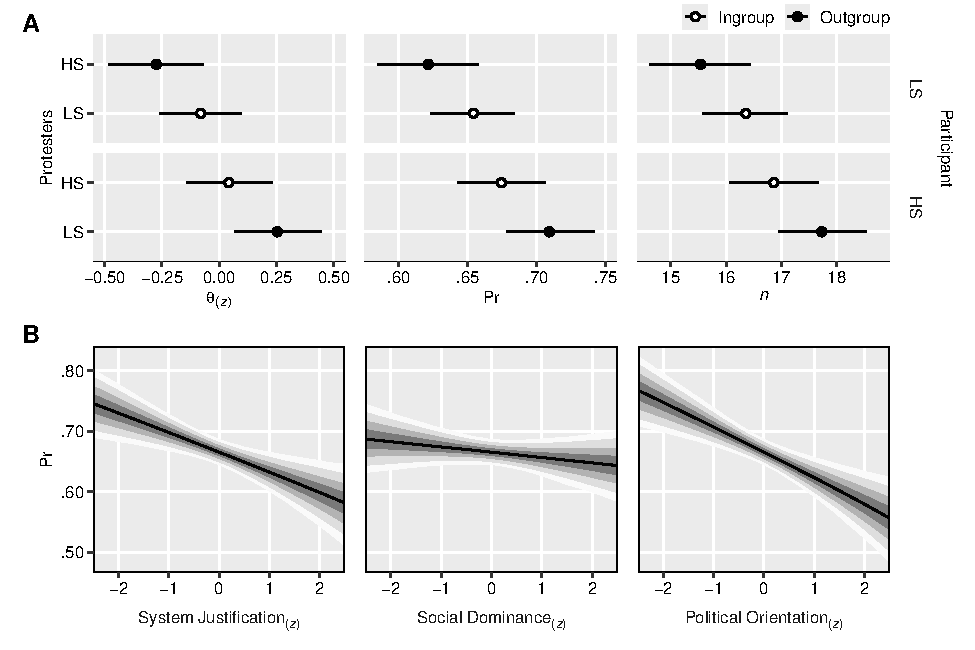
\includegraphics[scale=1]{../Experiment 1/figures/figure-3}
\caption*{\textit{Note.} HS = Higher Status, LS = Lower Status. $\theta_{(z)}$ is the \textit{z}-standardized tendency to consider more controversial actions acceptable means of protest. (\textbf{A}) $p$ and $n$ are, respectively, the predicted proportion and number of actions a participant would consider acceptable means of protest in each condition. Bars enclose the 95\% most plausible estimates. (\textbf{B}) Ribbons enclose, from the darkest to the lightest shade, the 50\%, 80\%, 95\%, and 99\% most plausible estimates.}
\label{fig:f3}
\end{figure*}

\hypertarget{reactions-to-the-manipulation}{%
\subsubsection{Reactions to the
Manipulation}\label{reactions-to-the-manipulation}}

Participants with professional jobs thought that they would be more
outraged if the government were to introduce a bill affecting people
with similar jobs (\(M = 6.00, SD = 1.05\)) than by a bill affecting
people with working-class jobs (\(M = 5.38, SD = 1.28\); Cohen's
\(d = 0.50\)). Conversely, participants with working-class jobs thought
that they would be more outraged by a bill affecting people in similar
jobs (\(M = 6.26, SD = 1.05\)) than by a bill affecting people in
professional jobs (\(M = 5.61, SD = 1.47\); \(d = 0.52\)). Participants
thought that a bill affecting people with similar jobs would affect them
personally (\(d = 1.14\)) and people like them (\(d = 1.33\)) more than
a bill affecting people with other jobs. Participants identified to a
greater extent with people in similar jobs (\(M = 6.21, SD = 1.12\))
than with people in other jobs (\(M = 4.06, SD = 1.65\); \(d = 1.22\)).
Overall, participants' reactions suggested that the experimental design
worked as intended and that participants in the lower-status and
higher-status groups understood the vignette in ingroup--outgroup terms.

\hypertarget{preregistered-analyses}{%
\subsubsection{Preregistered Analyses}\label{preregistered-analyses}}

To test our hypotheses, we estimated a two-parameter logistic item
response theory model (Bürkner, 2021) with participants' responses to
the question whether they thought each action was an acceptable means of
protest as the outcome variable. For each action \(i\), the model
estimated how acceptable (\(\beta_i\)) and discriminating (\(\alpha_i\))
that protest action was. For each participant \(j\), the model estimated
their unique propensity to consider protest actions acceptable
(\(\theta_j\)). In addition, the model estimated how accepting
participants were of controversial protest actions as a function of
three dummy-coded variables that encoded the group status of the
protesters and the participant.

We estimated this model in CmdStan (Gabry \& Cesnovar, 2021; Stan
Development Team, 2021) using Bayesian statistical methods. Bayesian
inference involves choosing a likelihood function and prior
distributions. A likelihood function links the observed data to the
model parameters and states how likely the observed data are given
different values of said model parameters. Prior distributions state how
plausible different values of said model parameters are before
considering the observed data. Bayesian inference applies Bayes' theorem
to update prior distributions in light of the observed data to produce
posterior distributions. In contrast to \(p\)-values and confidence
intervals, posterior distributions have a straight-forward
interpretation as stating how plausible different values of the model
parameters are given the observed data.

Our model derived the likelihood of participants' responses from a
Bernoulli likelihood function with a logistic regression equation
linking the two item parameters (\(\alpha_i\), \(\beta_i\)), the one
participant parameter (\(\theta_j\)), and the three regression
coefficients to the observed data. To identify the model, we constrained
\(\theta_j\) to have a mean of zero and constrained \(\alpha_i\) to have
a fixed mean and to be non-negative. We used partial pooling to estimate
\(\alpha_i\), \(\beta_i\), and \(\theta_j\). Our model assigned weakly
informative prior distributions (Gelman et al., 2017) to all model
parameters.\footnote{Our model assigned \(\text{Half-Cauchy} (0, 3)\)
  prior distributions to the standard deviations of \(\alpha_i\),
  \(\beta_i\), and \(\theta_j\) and \(\text{Normal} (0, 3)\) prior
  distributions to all other model parameters.} We report point
estimates, based on the median of posterior samples, and uncertainty
intervals, based on the quantiles of posterior samples, that enclose the
95\% most plausible estimates.

Figure \ref{fig:f3} (A) shows estimates for each combination of the
protesters' and the participants' group membership. Overall, we found
that participants' responses depended on both the protesters' and the
participants' group status---but not in the directions predicted by our
hypotheses. Contradicting our first hypothesis, participants did not
consider protest actions performed by their ingroup to be more
acceptable, on average, than the same actions performed by the relevant
outgroup (Cohen's \(d = 0.00, [-0.20, 0.20]\)). Instead, we found that
participants from higher-status backgrounds considered protest actions
performed by both lower-status (\(d = 0.34, [0.07, 0.59\){]}) and
higher-status (\(d = 0.33, [0.03, 0.63]\)) protesters to be, on average,
more acceptable than participants from lower-status backgrounds.
Contradicting our second hypothesis, participants considered protest
actions performed by higher-status protesters to be less acceptable, on
average, than the same actions performed by lower-status protesters
(\(d = -0.20, [-0.40, -0.00]\)).

\hypertarget{non-preregistered-analyses}{%
\subsubsection{Non-Preregistered
Analyses}\label{non-preregistered-analyses}}

We explored to what extent participants' ideological orientations
influenced how acceptable they considered various protest actions to be.
To that end, we estimated another two-parameter logistic item response
model that estimated participants' responses as a function of the
participant's and the protesters' group status and of the participants'
political orientation, social dominance orientation, and
system-justifying beliefs. We used factor scores to quantify social
dominance orientation and system-justifying beliefs and standardized all
new predictor variables. We report standardized regression coefficients
that quantify by how many standard deviations a participant's propensity
to consider more collective actions acceptable increases for each
additional standard deviation of the predictor variable.

Figure \ref{fig:f3} (B) the \(z\)-standardized propensity to consider
more controversial protest actions acceptable as a function of the three
ideological orientation variables. We found that participants who
reported a more right-wing political orientation
(\(\beta_{xy} = -0.25, [-0.37, -0.15]\)) and who expressed more
agreement with system-justifying beliefs
(\(\beta_{xy} = -0.20, [-0.30, -0.10]\)) tended to find fewer collective
actions to be acceptable. In contrast, we found that, after controlling
for the other two variables, social dominance orientation was not
associated with participants' judgements about how acceptable various
collective actions are (\(\beta_{xy} = -0.05, [-0.15, 0.05]\)). Overall,
these findings suggest that people who are right-wing and endorse
system-justifying beliefs tend to find various collective actions to be
less acceptable than people who are left-wing and do not endorse
system-justifying beliefs.\footnote{We ran additional analyses to
  explore how these associations differed across experimental
  conditions. We found uncertainty intervals for these associations to
  overlap across conditions, suggesting that we did not have enough data
  to differentiate these varying effects.}

\hypertarget{discussion}{%
\subsection{Discussion}\label{discussion}}

Experiment 1 provided a first test of the hypothesized identity- and
ideology-based double standards in judging collective action. That is,
we tested whether, in line with \emph{Hypothesis 1a} and \emph{1b},
participants would judge the same protest actions as more acceptable if
the protesters were ingroup members protesting for the ingroup's rights
or whether, in line with \emph{Hypothesis 2a}, participants would judge
the same protest actions as more acceptable if the protesters were from
a higher-status group. We found that participants' responses depended on
both the participants' and the protesters' group memberships---but not
in the hypothesized directions. Instead, we found that both lower-status
and higher-status participants tended to find the same protest actions
more acceptable when lower-status protesters protested a bill
threatening their rights. In non-preregistered analyses, we further
found that people who were right-wing and endorsed system-justifying
beliefs tended to find all protest actions to be less acceptable.

Experiment 1 did not, however, provide a conclusive test of our
hypotheses. First, by focusing on fictitious government bills, we might
have chosen a scenario too far removed from current affairs to evoke
strong ingroup bias in participants' judgements of protest actions. That
said, participants' reactions to the experimental manipulation suggested
that it evoked outrage and was understood in ingroup--outgroup terms.
Second, by focusing on collective action to defend workers' rights, we
arguably studied reactions to collective action for a progressive cause.
To test for ideology-based double standards, we relied on the assumption
that collective action by lower-status group members would be seen as
more challenging to the prevailing system than collective action by
higher-status group members. This assumption, however, was contradicted
by our observation that participants who endorsed system-justifying
beliefs tended to find actions by lower-status and higher-status
protesters to be less acceptable. Experiment 2 addressed those
limitations by focusing on a scenario we expected to evoke stronger
responses from participants and by examining reactions to both
system-challenging and system-defending collective action.

\hypertarget{experiment-2}{%
\section{Experiment 2}\label{experiment-2}}

In Experiment 2, we investigated potential double standards in judging
collective action for or against defunding the police in the United
States. That is, we tested whether Black and White Americans applied
different standards when judging collective action taken by either Black
or White protesters to protest either for or against police divestment
as a possible solution to racist police violence. We conducted this
study in January 2021, a time when, after a year of unprecedented
protests for racial justice, most Americans could be expected to be
aware of, and have formed an opinion on, the Black Lives Matter
movement. We focused on defunding the police as this position remained
controversial among both Black and White Americans even as they broadly
agreed on the need for police reform.\footnote{In December 2020, only
  34\% of Black Americans and 18\% of White Americans supported
  defunding the police while majorities of Black and White Americans
  supported police reforms such as eliminating qualified immunity (50\%
  and 57\%) or banning chokeholds (79\% and 61\%, YouGov, 2020).}

By varying the participants' and the protesters' group memberships, we
tested the preregistered hypothesis that participants would judge the
same protest actions as more acceptable if the protesters were ingroup
members (\emph{Hypothesis 1a}). By assuming that defunding the police
aligns more closely with the interests of Black than White Americans, we
tested the preregistered hypothesis that participants would judge the
same protest actions as more acceptable if the cause of the protest
aligned with their ingroup's interests (\emph{Hypothesis 1b}). By
varying whether the protesters protested for or against defunding the
police, we tested the preregistered hypotheses that participants would
judge the same protest actions as more acceptable if the protest
supported, rather than challenged, the system (\emph{Hypothesis 2a}) and
if they endorsed system-justifying beliefs and the protest supported the
system or if they rejected system-justifying beliefs and the protest
challenged the system (\emph{Hypothesis 2b}). In this way, Experiment 2
provided a complete test of the hypothesized identity- and
ideology-based double standards in judging collective action. In
addition, we tested the simpler, alternative hypothesis that
participants, in general, would judge the same protest actions as more
acceptable if they supported the protesters' cause (\emph{Hypothesis
3}).

\hypertarget{method-1}{%
\subsection{Method}\label{method-1}}

We preregistered the sample size as well as all hypotheses,
inclusion/exclusion criteria, measures, and manipulations
(\url{https://osf.io/skxjt/?view_only=d8ce44a700884b5ab36b64ef08f833a1}).
We made all materials, data, and analysis scripts available online
(\url{https://osf.io/d3yev/?view_only=40782034017c40f0bcecb1cc87760b62}).
As reported in the preregistration, we ran simulations, using data from
Experiment 1, to determine that a sample size of \(N = 1,600\)
(\(n = 200\) per condition) was sufficient to detect even small
differences between conditions (\(0.09 < \text{Cohen's}~d < 0.16\)).

\hypertarget{study-design-1}{%
\subsubsection{Study Design}\label{study-design-1}}

We used a 2 (quasi-experimental: Black/White participants) \(\times\) 2
(experimental: Black/White protesters) \(\times\) 2 (experimental:
for/against defunding the police) between-subjects design to test our
hypotheses.

\hypertarget{participants-1}{%
\subsubsection{Participants}\label{participants-1}}

We recruited 1,773 Black and White American participants from the
Prolific subject pool who were 18 years old or older, lived in the US,
and were US citizens.\footnote{Data were collected between January 15
  and 28, 2021. Participants received, on average, \$12.89 per hour of
  participation.} As preregistered, we excluded 173 participants who
failed at least one of three attention checks or who reported a
different ethnic background than they had reported in the Prolific
prescreening questionnaire. This resulted in a final sample of 1,600
participants (\(\textit{Mdn} = 31\) years, age range: 18--84 years; 864
women, 708 men, 27 sex/gender diverse) of whom 800 identified as Black
and 800 identified as White.

\hypertarget{procedure-1}{%
\subsubsection{Procedure}\label{procedure-1}}

Participants read the following paragraphs:

\begin{quote}
In 2020, police officers killed Breonna Taylor and George Floyd. Many
were outraged that police officers had, once again, killed unarmed Black
Americans. Across the United States, people called for changes to
prevent future police violence.
\end{quote}

\begin{quote}
Some argue that, to end police violence, we should take money away from
police departments. Reducing police funding would mean fewer police
officers on the street. Fewer police officers would mean fewer
opportunities for them to turn violent. Reducing police funding would
also leave more money for other services. Proponents argue for
reallocating police funding to social services, housing, and education.
Doing so would keep communities safer with fewer police officers. We
refer to this position as ``defunding the police''. This position
differs from ``reforming the police'' which might mean increasing police
funding and also differs from ``abolishing the police'' which means
disbanding police departments altogether.
\end{quote}

\noindent Participants were then asked to answer whether the text had
been about ``reforming the police'', ``defunding the police'', or
``abolishing the police''. If they selected the wrong answer, they were
instructed to reread the text and select the right answer. On the next
page, participants stated whether they supported or opposed the proposed
solution.

Participants in the system-challenging protest condition then read a
text about protesters in support of defunding the police:

\begin{quote}
Earlier, you read about defunding the police as a possible solution to
end police violence. Some local residents want to protest for defunding
the police. They argue that reducing police funding would prevent police
violence.
\end{quote}

\noindent Participants in the system-supporting protest condition
instead read about protesters rallying against defunding the police:

\begin{quote}
Some local residents want to protest against defunding the police. They
argue that reducing police funding would mean fewer police officers
serving their community.
\end{quote}

\noindent Participants then read either that ``most of the protesters
are Black'' or that ``most of the protesters are White''. Participants
again had to correctly answer multiple choice questions about the text
(``Are the protesters for or against defunding the police?'', ``Who are
the protesters?'') before being able to proceed.

On the next pages, participants completed all remaining measures. On the
final page, participants responded to three attention checks: ``In this
study, you first read about a proposed solution to police violence. What
was it?'' (\emph{reforming the police}, \emph{defunding the police},
\emph{abolishing the police}); ``In this study, you then read about
protesters. Were these protesters for or against the proposed
solution?'' (\emph{for}, \emph{against}); and ``Were most of the
protesters Black or White?'' (\emph{Black}, \emph{White}). As
preregistered, we excluded participants who gave an answer inconsistent
with their assigned experimental condition.

\hypertarget{measures-1}{%
\subsubsection{Measures}\label{measures-1}}

We measured the outcome variable by asking participants to think about
the protesters they had read about and to decide, for each of 25 protest
actions presented in a randomized order, whether they thought this
action was ``an acceptable means for them to protest {[}for/against{]}
defunding the police'' (1 = \emph{yes}, 0 = \emph{no}). We replaced some
actions from Experiment 1 because they either did not fit the study
context or had been considered acceptable by almost all participants
(see Table B1).

We measured system-justifying beliefs with eight items (adapted from Kay
\& Jost, 2003), for example, ``in general, I find society to be fair''
(1 = \emph{strongly disagree}, 7 = \emph{strongly agree}; McDonald's
\(\omega = .91\)). A confirmatory factor analysis model in which all
items loaded onto a single factor showed acceptable fit,
\(\chi^2 (28) = 4309.15; \text{CFI} = 0.95; \text{TLI} = 0.93; \text{RMSEA} = 0.11, [0.10, 0.12]\).

We measured support for defunding the police with one item: ``Do you
support or oppose defunding the police?'' (1 = \emph{strongly oppose}, 5
= \emph{strongly support}).

We included additional measures to describe the sample, to describe
reactions to the manipulation, or to use in non-preregistered analyses.
In addition to demographic questions, we asked participants how outraged
they were about recent incidents of police violence against Black
Americans, to what extent they identifed with the protesters described
in the study, and to what extent they identifed with their racial
ingroup (1 = \emph{not at all}, 7 = \emph{very much}). We also asked how
often, if at all, participants had participated in protest actions such
as the ones we had asked about (1 = \emph{never}, 5 = \emph{very often})
and whether they has participated in protests for reforming, defunding
or abolishing the police; against reforming, defunding or abolishing the
police; or in neither. We measured political orientation with a one-item
semantic differential scale: ``People often describe their political
orientation as liberal or conservative. On a scale from liberal to
conservative, where would you position yourself?'' (1 = \emph{liberal},
7 = \emph{conservative}).

\hypertarget{results-1}{%
\subsection{Results}\label{results-1}}

\begin{figure*}[!t]
\centering
\caption{Results from the preregistered analyses for Experiment 2}
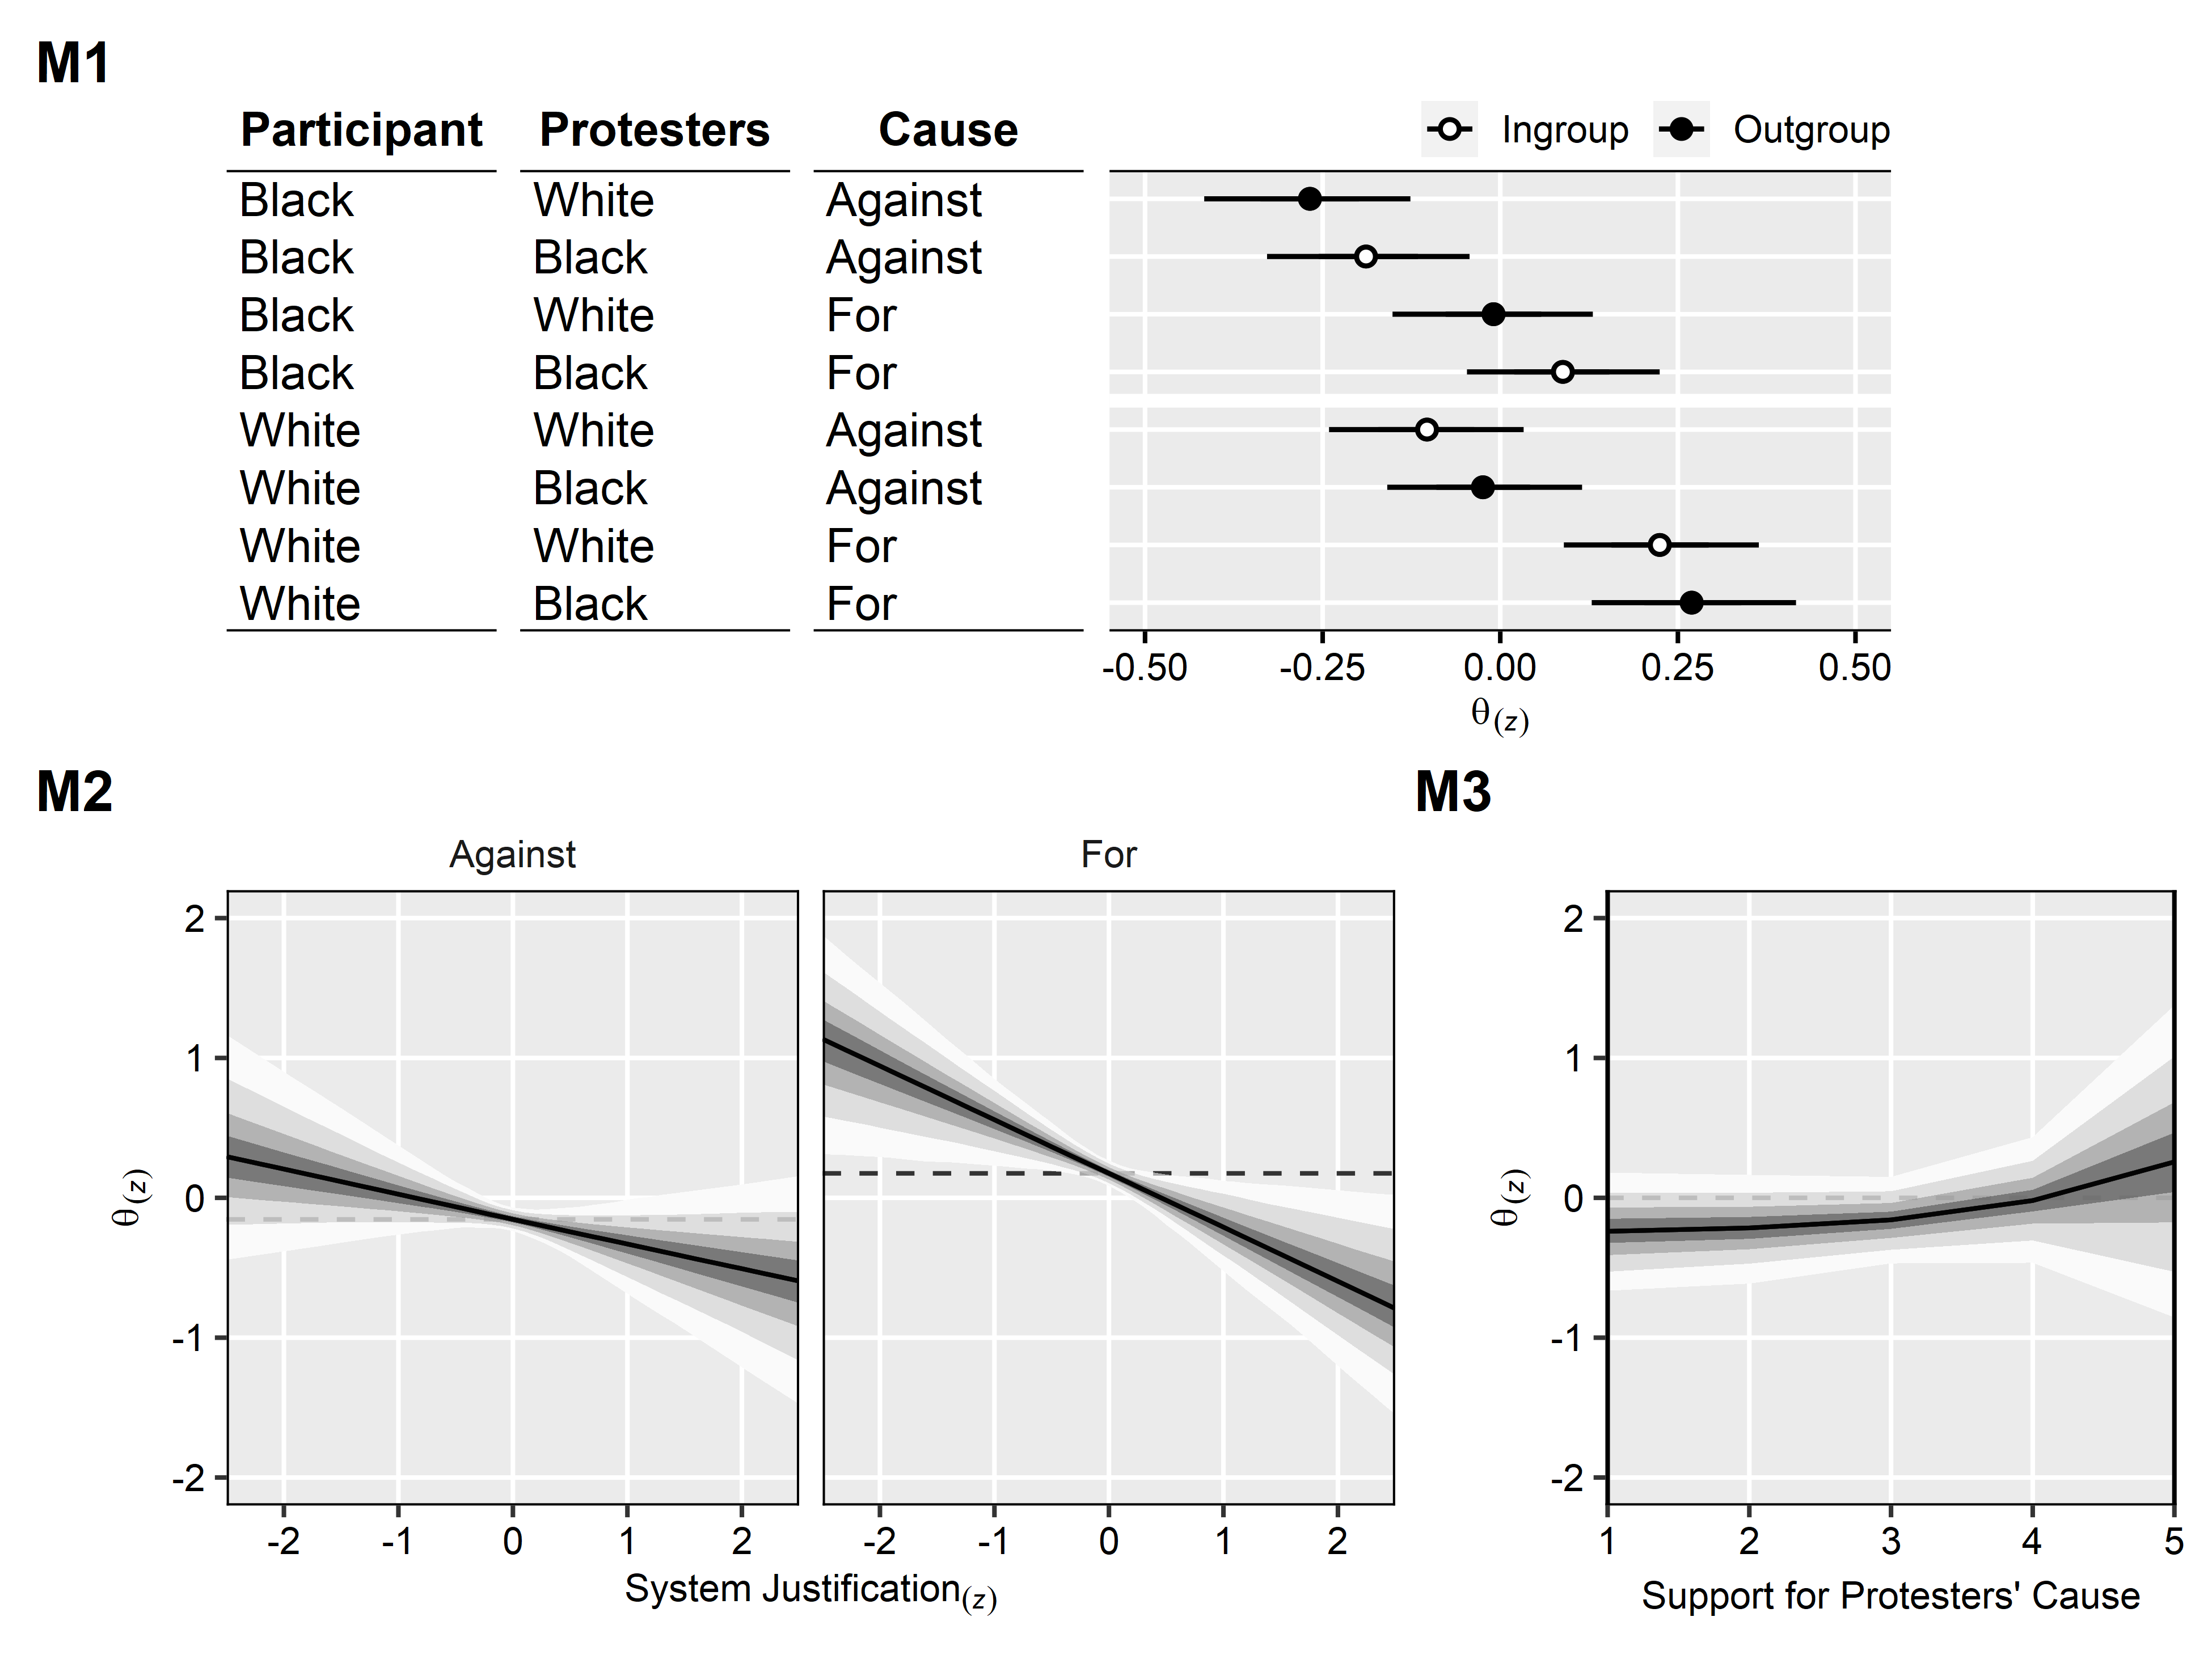
\includegraphics[scale=1]{../Experiment 2/figures/figure-4}
\caption*{\textit{Note.} Against = Protesters oppose defunding the police. For = Protesters support defunding the police. $\theta_{(z)}$ is the \textit{z}-standardized tendency to consider more controversial actions acceptable means of protest. Ribbons enclose, from the darkest to the lightest shade, the 50\%, 80\%, 95\%, and 99\% most plausible estimates.}
\label{fig:f4}
\end{figure*}

\begin{figure*}[!t]
\centering
\caption{Predictions from the preregistered (system justification) and non-preregistered (political orientation) analyses for Experiment 2}
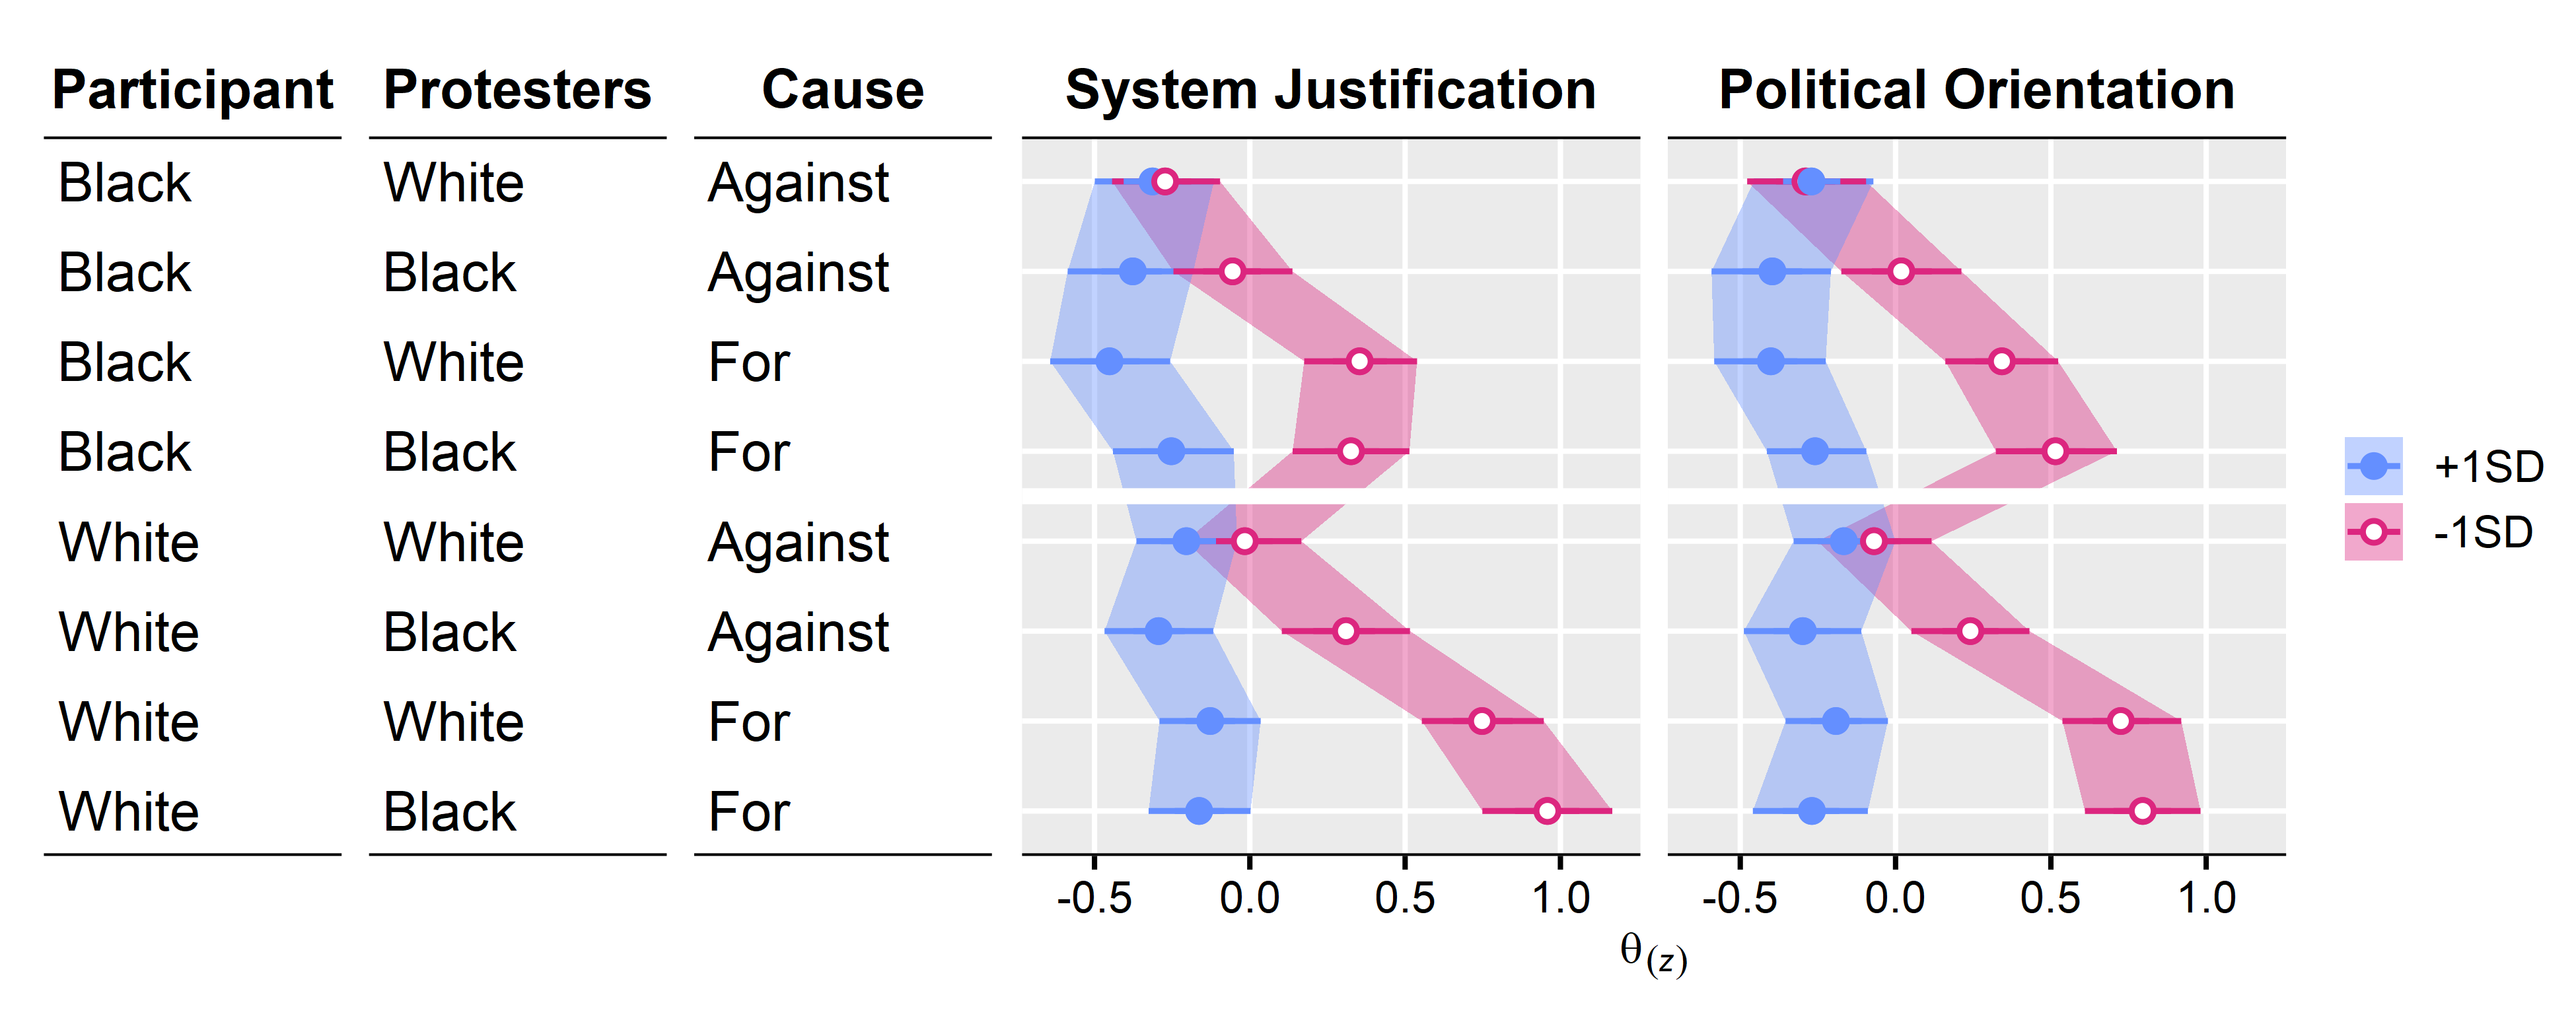
\includegraphics[scale=1]{../Experiment 2/figures/figure-5}
\caption*{\textit{Note.} Against = Protesters oppose defunding the police. For = Protesters support defunding the police. $\theta_{(z)}$ is the \textit{z}-standardized tendency to consider more controversial actions acceptable means of protest.}
\label{fig:f5}
\end{figure*}

\hypertarget{reactions-to-the-manipulation-1}{%
\subsubsection{Reactions to the
Manipulation}\label{reactions-to-the-manipulation-1}}

As expected, Black participants (\(M = 6.18, \textit{SD} = 1.31\))
reported being more outraged about recent incidents of police violence
than White participants (\(M = 5.56, \textit{SD} = 1.61\); Cohen's
\(d = 0.42\)). Black participants strongly identified with their ingroup
(\(M = 6.46, \textit{SD} = 1.09\)) and, across experimental conditions,
identified more with Black protesters (\(M = 4.66, \textit{SD} = 1.99\))
than with White protesters (\(M = 4.03, \textit{SD} = 2.16\);
\(d = 0.30\)). In contrast, White participants identified less strongly
with their ingroup (\(M = 4.85, \textit{SD} = 1.53\); \(d = 1.21\)) and
did not identify more with White protesters
(\(M = 3.58, \textit{SD} = 2.01\)) than with Black protesters
(\(M = 3.81, \textit{SD} = 1.77\); \(d = -0.12\)). Both White
(\(d = 0.67\)) and Black (\(d = 0.53\)) participants tended to identify
more with protesters protesting \emph{for} defunding the police. On
average, participants tended to describe their political orientation as
moderately liberal (\(M = 2.92, \textit{SD} = 1.73\)) but, as expected,
were divided in their support for defunding the police
(\(M = 3.37, \textit{SD} = 1.42\)). That is, 56\% supported defunding
the police, 30\% opposed defunding the police, and 14\% remained
undecided.

\hypertarget{preregistered-analyses-1}{%
\subsubsection{Preregistered Analyses}\label{preregistered-analyses-1}}

To test our hypotheses, we estimated a series of two-parameter logistic
item response theory models with participants' responses to the question
whether they thought each action was an acceptable means of protest as
the outcome variable. Our models differed from the models used in
Experiment 1 in two ways. First, we estimated the item parameters
(\(\alpha_i\), \(\beta_i\)) as \emph{correlated} varying effects.
Second, we used varying, rather than fixed, effects to estimate
differences between the eight conditions. This resulted in partial
pooling---condition-wise estimates were shrunk towards each other---and
allowed us to compare conditions without multiple comparison problems
(Gelman et al., 2012). Our models assigned weakly informative prior
distributions to all model parameters.\footnote{Our model assigned
  \(\text{LKJ} (2)\) prior distributions to the Cholesky-transformed
  correlation matrices for varying effects and
  \((\text{Half-})\text{Cauchy} (0, 5)\) prior distributions to all
  other model parameters.} Figure \ref{fig:f4} shows results from three
preregistered models we estimated to test our hypotheses.

Model 1 (M1) estimated varying intercepts for the eight conditions to
test whether, in line with Hypotheses 1a, 1b, or 2a, participants'
responses depended on their own group membership, the protesters' group
membership, or the protesters' cause. Contradicting \emph{Hypothesis
1a}, participants did not consider protest actions performed by their
ingroup to be more acceptable, on average, than the same actions
performed by the relevant outgroup (\(d = 0.01, [-0.04, 0.06]\)).
Contradicting \emph{Hypothesis 1b}, participants did not consider
protest actions for a cause that was nominally aligned with their
ingroup's interests to be more acceptable, on average, than protest
actions for a cause not aligned with their ingroup's interests
(\(d = -0.01, [-0.06, 0.04]\)). Contradicting \emph{Hypothesis 2a},
participants did not consider protest actions for a system-defending
cause to be more acceptable, on average, than protest actions for a
system-challenging cause (\(d = -0.14, [-0.20, -0.09]\)). Instead, we
found that, on average, White participants considered all protest
actions to be more acceptable than Black participants
(\(d = 0.09, [0.04, 0.14]\)) and both Black (\(d = 0.07, [0.03, 0.10]\))
and White (\(d = 0.08, [0.04, 0.11]\)) participants considered the same
actions to be more acceptable when protests were for, rather than
against, defunding the police. As in Experiment 1, we thus found that
participants' responses depended on both the participants' and the
protesters' group memberships---but not in the directions predicted by
our hypotheses.

Model 2 (M2) extended Model 1 by estimating participants' responses as a
function of their \emph{z}-standardized endorsement of system-justifying
beliefs. As preregistered, we modeled this relationship with two fixed
effects, one estimating the effect of system-justifying beliefs on
judgements about system-defending protest actions and one estimating
their effect on judgements about system-challenging protest actions, and
one varying effect estimating its variance across conditions. Supporting
\emph{Hypothesis 2b}, participants who \emph{rejected} system-justifying
beliefs were \emph{more} likely to consider system-challenging protest
actions (for defunding the police) to be acceptable means of protest
(\(\beta_{xy} = 0.38, [0.16, 0.58]\)). We did not, however, find
evidence for the ideological symmetry implied by \emph{Hypothesis 2b}
since participants who \emph{endorsed} system-justifying beliefs were
\emph{not} more likely to consider system-defending protest actions
(against defunding the police) to be acceptable means of protest
(\(\beta_{xy} = -0.18, [-0.40, 0.02]\)).

Figure \ref{fig:f5} shows the estimated pattern of condition-wise
differences underlying those fixed effects. Participants who endorsed
system-justifying beliefs tended to consider system-challenging and
system-defending protest actions to be equally unacceptable. In
contrast, participants who rejected system-justifying beliefs evinced
ideology-based double standards: In line with \emph{Hypothesis 2b}, they
considered the same protest actions to be more acceptable when the
protesters challenged the system or, to a lesser extent, when the
protesters were from the disadvantaged group.

Model 3 (M3) extended Model 1 by estimating participants' responses as a
function of their self-reported support for the cause of the protest. We
recoded participants' responses to create a predictor variable that
encoded support for defunding the police when protesters supported
defunding the police and opposition to defunding the police when
protesters opposed defunding the police. As preregistered, we modeled
this relationship as a monotonic effect (Bürkner \& Charpentier, 2020)
that estimated the average change in the outcome variable across
predictor categories as well as how much of this change occurred between
each of the four pairs of adjacent predictor categories.\footnote{Our
  model assigned a Dirichlet prior, \(\alpha = {1, 1, 1, 1}\), to the
  proportions of the overall change that was expected to occur between
  each of the four pairs of predictor categories.} Contradicting
\emph{Hypothesis 3}, participants who supported the protesters' cause
did not, on average, consider the same protest actions to be more
acceptable than participants who opposed the protesters' cause
(\(\beta_{y} = 0.14, [-0.12, 0.40]\)). Ergo, our results did not support
the alternative hypothesis that ideology-based double standards can be
reduced to support for, or opposition to, the cause of a protest.

\hypertarget{non-preregistered-analyses-1}{%
\subsubsection{Non-Preregistered
Analyses}\label{non-preregistered-analyses-1}}

We explored whether group identification moderated how the participants'
and the protesters' group memberships affected participants' responses.
To that end, we extended Model 1 by estimating participants' responses
as a function of their \emph{z}-standardized identification with their
racial ingroup. As in Model 2, we modeled this relationship with a fixed
and a varying effect. We found, however, that even participants who
strongly identified with their racial ingroup (+1\emph{SD}) did not
consider protest actions performed by their ingroup to be more
acceptable than the same actions performed by the relevant outgroup
(\(d = 0.02, [-0.04, 0.07]\)) and did not consider protest actions for a
cause that was aligned with their ingroup's interests to be more
acceptable than protest actions for a cause not aligned with their
ingroup's interests (\(d = -0.03, [-0.09, 0.02]\)). Our
non-preregistered analyses thus suggested that group identification did
not moderate group differences in judgements about collective action by
ingroup and outgroup members.

We also explored whether we would find ideology-based double standards
when operationalizing ideology as political orientation instead of as
system justification. To that end, we reran Model 2 with political
orientation as the \emph{z}-standardized predictor variable. Our results
mirrored the preregistered analyses: More liberal participants were more
likely to consider protest actions for defunding the police to be
acceptable (\(\beta_{xy} = 0.41, [0.17, 0.62]\)) but more conservative
participants were not more likely to consider protest actions against
defunding the police to be acceptable
(\(\beta_{xy} = -0.16, [-0.41, 0.04]\)). As Figure 5 shows, conservative
participants tended to consider all protest actions to be equally
unacceptable while liberal participants considered the same protest
actions to be more acceptable when protesters rallied around a
progressive cause. Our non-preregistered analyses thus replicated the
ideology-based double standards from the preregistered analyses with a
different operationalization of ideology.

\hypertarget{discussion-1}{%
\subsection{Discussion}\label{discussion-1}}

Experiment 2 provided a complete test of the hypothesized identity- and
ideology-based double standards in judging collective action. As in
Experiment 1, we found that participants' responses depended on both the
participants' and the protesters' group memberships---but not in the
hypothesized directions. We found that, contrary to \emph{Hypothesis
1a}, participants considered protest actions taken by ingroup and
outgroup members to be equally acceptable and that, contrary to
\emph{Hypothesis 1b}, participants did not consider the same protest
actions to be more acceptable when the protesters' cause aligned with
their ingroup's interests. Like Experiment 1, Experiment 2 thus found no
evidence for identity-based double standards---even though it focused on
an issue of direct and current relevance to the participants.

Expanding Experiment 1, Experiment 2 considered reactions to both
system-challenging and system-defending collective action and, in so
doing, provided a stronger test of the hypothesized ideology-based
double standards. Contrary to \emph{Hypothesis 2a} and the underlying
assumption of a universal system-justifying motive, we found that
participants considered the same protest actions to be \emph{more}
acceptable when judging system-challenging collective action (for
defunding the police) than when judging system-defending collective
action. This finding might reflect our liberal-leaning sample. In line
with \emph{Hypothesis 2b}, we found that participants who rejected
system-justifying beliefs considered the same protest action more
acceptable when judging system-challenging collective action (for
defunding the police). We did not, however, find evidence for
ideological symmetry in this relationship as participants who endorsed
system-justifying beliefs considered system-challenging and
system-defending collective action to be equally unacceptable. In
addition, we did not find evidence for the alternative, simpler
\emph{Hypothesis 3} that that participants would judge the same protest
actions to be acceptable when they supported the protesters' cause. In
this way, Experiment 2 provided evidence for ideology-based, but not for
identity-based, double standards in judging collective action.

\hypertarget{general-discussion}{%
\section{General Discussion}\label{general-discussion}}

Our research was motivated by real-world examples that seemed to suggest
that where people draw the line between acceptable and unacceptable
protest actions depends on \emph{who} the protesters are and \emph{what}
they are protesting---in other words, that there are double standards in
judging collective action. Our findings, however, showed that it is not
so simple. Contradicting our hypothesis of identity-based double
standards, participants in two preregistered experiments did not show
ingroup bias when judging controversial protest actions taken by ingroup
and outgroup members to advance their group's interests. Instead,
supporting our hypothesis of ideology-based double standards,
participants judged the same controversial protest actions to be more
acceptable when the protesters' cause aligned with their own
(system-challenging) ideological position. In the remainder of this
General Discussion, we discuss theoretical and practical implications
for understanding the often divided response to collective action and
consider some limiting conditions on our findings.

\hypertarget{implications}{%
\subsection{Implications}\label{implications}}

Our results showed that, for many controversial protest actions, there
is no consensus on what is and is not an acceptable means to advance a
cause. Instead, this judgement seems to depend on what the cause of a
protest is and how it aligns with one's beliefs and values. In this way,
our results confirm our contention that the distinction between
normative and non-normative forms of collective action should be
situated in the eye of the beholder. By developing an instrument for
measuring where people draw the line between acceptable and unacceptable
forms of collective action, we provided a paradigm that we hope will
stimulate research on when and why people differ in making this
distinction.

After all, this distinction can be consequential. If people believe that
even extreme actions are acceptable means to advance a cause they
support, especially if they moralize their support for that cause
(Mooijman et al., 2018), they might support violent extremism. In this
way, our findings could explain why 45\% of Republicans (2\% of
Democrats) supported the storming of the U.S. Capitol on January 6, 2021
(YouGov, 2021) even though it was illegal, destructive, and violent. If
people believe that even non-violent actions are unacceptable means to
advance a cause they oppose, they might support stifling dissent. In
this way, our findings could explain why Republicans responded to Black
Lives Matter protests by seeking to further criminalize disruptive
protest (e.g., blocking highways, Quinton, 2021) that might be most
effective at challenging injustice (Shuman et al., 2022, 2021). For
those reasons, researchers should further investigate when and why
people apply different standards when judging collective action for
various causes.

\hypertarget{limitations}{%
\subsection{Limitations}\label{limitations}}

Our research applied item response theory to judgements about collective
action to investigate whether where people draw the line between
acceptable and unacceptable means of protest depends on who the
protesters are and what they are protesting. In so doing, we moved the
distinction between normative and non-normative collective action from
the realm of the researcher's intuition into the realm of scientific
investigation, allowing us to test for double standards in judging
collective action.

Despite its strengths, our research is qualified by several limitations.
First, our research examined the hypothesized relationships for only two
political causes---protecting workers' rights, defunding the
police---and thus provided only limited evidence that our findings
generalize beyond those causes. Relying on few stimuli to establish an
effect threatens the validity and replicability of research findings and
severely constrains psychological research generalize beyond those few
stimuli (Yarkoni, 2022). Future research should sample a wider range of
causes to address this pervasive but often ignored problem (Judd et al.,
2012). This is particularly important when studying collective action as
recent theorizing (Jost et al., 2017) and research (Osborne et al.,
2019) highlighted the importance of differentiating between progressive
and conservative causes. Second, our research was based on two Western,
Educated, Industrialized, Rich, and Democratic (WEIRD; Henrich et al.,
2010) samples, which severely limits the cross-cultural generalizability
of our findings. Future research should include samples from a wider
range of cultural context to examine how the observed relationships vary
across cultural contexts.

\hypertarget{conclusion}{%
\section{Conclusion}\label{conclusion}}

Opinion polls show deep divides not only about the ends of protests, but
also about the means of protest. For example, only 11\% of Republicans
and 29\% of White Americans---compared to 59\% of Democrats and 66\% of
Black Americans---considered kneeling during the national anthem---a
non-violent form of collective action---an appropriate means to protest
racist police violence (YouGov, 2017). Our research showed that, in
contrast to well-documented double standards in other domains, people do
not apply a different standard when judging collective action by ingroup
members or for a cause aligned with the ingroup's interests. Instead,
our research demonstrated that people consider the same protest actions
to be more acceptable when the cause of the protest aligns with their
own ideological positions---in other words, that there are partisan
double standards in judging collective action.

\refsection

\begingroup

\noindent \setlength{\parindent}{-0.5in} \setlength{\leftskip}{0.5in}
\small

\hypertarget{refs}{}
\begin{CSLReferences}{1}{0}
\leavevmode\vadjust pre{\hypertarget{ref-abrams_double_2013}{}}%
Abrams, D., Randsley de Moura, G., \& Travaglino, G. A. (2013). A double
standard when group members behave badly: {Transgression} credit to
ingroup leaders. \emph{Journal of Personality and Social Psychology},
\emph{105}(5), 799--815. \url{https://doi.org/10.1037/a0033600}

\leavevmode\vadjust pre{\hypertarget{ref-becker_virtual_2012}{}}%
Becker, J. C. (2012). Virtual special issue on theory and research on
collective action in the {European} {Journal} of {Social} {Psychology}
{[}{Editorial}{]}. \emph{European Journal of Social Psychology},
\emph{42}(1), 19--23. \url{https://doi.org/10.1002/ejsp.1839}

\leavevmode\vadjust pre{\hypertarget{ref-becker_committed_2011}{}}%
Becker, J. C., Tausch, N., Spears, R., \& Christ, O. (2011). Committed
dis(s)idents: {Participation} in radical collective action fosters
disidentification with the broader in-group but enhances political
identification. \emph{Personality and Social Psychology Bulletin},
\emph{37}(8), 1104--1116. \url{https://doi.org/10.1177/0146167211407076}

\leavevmode\vadjust pre{\hypertarget{ref-brewer_social_2007}{}}%
Brewer, M. B. (2007). The social psychology of intergroup relations:
Social categorization, ingroup bias, and outgroup prejudice. In A. W.
Kruglanski \& E. T. Higgins (Eds.), \emph{Social psychology: Handbook of
basic principles} (2nd ed., pp. 695--715). Guilford Press.

\leavevmode\vadjust pre{\hypertarget{ref-burkner_bayesian_2021}{}}%
Bürkner, P.-C. (2021). Bayesian item response modeling in {R} with brms
and {Stan}. \emph{Journal of Statistical Software}, \emph{100}(5).
\url{https://doi.org/10.18637/jss.v100.i05}

\leavevmode\vadjust pre{\hypertarget{ref-burkner_modelling_2020}{}}%
Bürkner, P.-C., \& Charpentier, E. (2020). Modelling monotonic effects
of ordinal predictors in {Bayesian} regression models. \emph{British
Journal of Mathematical and Statistical Psychology}, \emph{73}(3),
420--451. \url{https://doi.org/10.1111/bmsp.12195}

\leavevmode\vadjust pre{\hypertarget{ref-demars_irt_2010}{}}%
DeMars, C. (2010). \emph{Item response theory}. Oxford University Press.

\leavevmode\vadjust pre{\hypertarget{ref-dunivin_black_2022}{}}%
Dunivin, Z. O., Yan, H. Y., Ince, J., \& Rojas, F. (2022). Black {Lives}
{Matter} protests shift public discourse. \emph{Proceedings of the
National Academy of Sciences}, \emph{119}(10), e2117320119.
\url{https://doi.org/10.1073/pnas.2117320119}

\leavevmode\vadjust pre{\hypertarget{ref-endevelt_everyone_2021}{}}%
Endevelt, K., Schori-Eyal, N., \& Halperin, E. (2021). Everyone should
get the same, but we should get more: Group entitlement and intergroup
moral double standard. \emph{Group Processes \& Intergroup Relations},
\emph{24}(3), 350--370. \url{https://doi.org/10.1177/1368430219896618}

\leavevmode\vadjust pre{\hypertarget{ref-feinberg_activists_2020}{}}%
Feinberg, M., Willer, R., \& Kovacheff, C. (2020). The activist's
dilemma: {Extreme} protest actions reduce popular support for social
movements. \emph{Journal of Personality and Social Psychology},
\emph{119}(5), 1086--1111. \url{https://doi.org/10.1037/pspi0000230}

\leavevmode\vadjust pre{\hypertarget{ref-foschi_double_2000}{}}%
Foschi, M. (2000). Double standards for competence: Theory and research.
\emph{Annual Review of Sociology}, \emph{26}(1), 21--42.
\url{https://doi.org/10.1146/annurev.soc.26.1.21}

\leavevmode\vadjust pre{\hypertarget{ref-cmdstanr_2021}{}}%
Gabry, J., \& Cesnovar, R. (2021). \emph{{cmdstanr}: {R} interface to
{CmdStan}} (Version 0.4.0). \url{https://mc-stan.org/cmdstanr}

\leavevmode\vadjust pre{\hypertarget{ref-gelman_why_2012}{}}%
Gelman, A., Hill, J., \& Yajima, M. (2012). Why we (usually) don't have
to worry about multiple comparisons. \emph{Journal of Research on
Educational Effectiveness}, \emph{5}(2), 189--211.
\url{https://doi.org/10.1080/19345747.2011.618213}

\leavevmode\vadjust pre{\hypertarget{ref-gelman_prior_2017}{}}%
Gelman, A., Simpson, D., \& Betancourt, M. (2017). The prior can often
only be understood in the context of the likelihood. \emph{Entropy},
\emph{19, 10}, 555. \url{https://doi.org/10.3390/e19100555}

\leavevmode\vadjust pre{\hypertarget{ref-hewstone_ultimate_1990}{}}%
Hewstone, M. (1990). The {``ultimate attribution error''}? {A} review of
the literature on intergroup causal attribution. \emph{European Journal
of Social Psychology}, \emph{20}(4), 311--335.
\url{https://doi.org/10.1002/ejsp.2420200404}

\leavevmode\vadjust pre{\hypertarget{ref-ho_nature_2015}{}}%
Ho, A. K., Sidanius, J., Kteily, N., Sheehy-Skeffington, J., Pratto, F.,
Henkel, K. E., Foels, R., \& Stewart, A. L. (2015). The nature of social
dominance orientation: {Theorizing} and measuring preferences for
intergroup inequality using the new {SDO}-7 scale. \emph{Journal of
Personality and Social Psychology}, \emph{109}(6), 1003--1028.
\url{https://doi.org/10.1037/pspi0000033}

\leavevmode\vadjust pre{\hypertarget{ref-jost_theory_2020}{}}%
Jost, J. T. (2020). \emph{A theory of system justification}. Harvard
University Press.

\leavevmode\vadjust pre{\hypertarget{ref-jost_role_1994}{}}%
Jost, J. T., \& Banaji, M. R. (1994). The role of stereotyping in
system-justification and the production of false consciousness.
\emph{British Journal of Social Psychology}, \emph{33}(1), 1--27.
\url{https://doi.org/10.1111/j.2044-8309.1994.tb01008.x}

\leavevmode\vadjust pre{\hypertarget{ref-jost_missing_2017}{}}%
Jost, J. T., Becker, J., Osborne, D., \& Badaan, V. (2017). Missing in
(collective) action: Ideology, system justification, and the
motivational antecedents of two types of protest behavior. \emph{Current
Directions in Psychological Science}, \emph{26}(2), 99--108.
\url{https://doi.org/10.1177/0963721417690633}

\leavevmode\vadjust pre{\hypertarget{ref-jost_political_2003}{}}%
Jost, J. T., Glaser, J., Kruglanski, A. W., \& Sulloway, F. J. (2003).
Political conservatism as motivated social cognition.
\emph{Psychological Bulletin}, \emph{129}(3), 339--375.
\url{https://doi.org/10.1037/0033-2909.129.3.339}

\leavevmode\vadjust pre{\hypertarget{ref-judd_treating_2012}{}}%
Judd, C. M., Westfall, J., \& Kenny, D. A. (2012). Treating stimuli as a
random factor in social psychology: {A} new and comprehensive solution
to a pervasive but largely ignored problem. \emph{Journal of Personality
and Social Psychology}, \emph{103}(1), 54--69.
\url{https://doi.org/10.1037/a0028347}

\leavevmode\vadjust pre{\hypertarget{ref-kay_complementary_2003}{}}%
Kay, A. C., \& Jost, J. T. (2003). Complementary justice: Effects of
"poor but happy" and "poor but honest" stereotype exemplars on system
justification and implicit activation of the justice motive.
\emph{Journal of Personality and Social Psychology}, \emph{85}(5),
823--837. \url{https://doi.org/10.1037/0022-3514.85.5.823}

\leavevmode\vadjust pre{\hypertarget{ref-lacina_nfl_2020}{}}%
Lacina, B. (2020). \emph{National anthem protests and whites' views of
black NFL players} {[}Unpublished manuscript{]}. Department of Political
Science, University of Rochester.
\url{http://www.bethanylacina.com/docs/Lacina_NFL_paper.pdf}

\leavevmode\vadjust pre{\hypertarget{ref-mendoza_for_2014}{}}%
Mendoza, S. A., Lane, S. P., \& Amodio, D. M. (2014). For members only:
Ingroup punishment of fairness norm violations in the ultimatum game.
\emph{Social Psychological and Personality Science}, \emph{5}(6),
662--670. \url{https://doi.org/10.1177/1948550614527115}

\leavevmode\vadjust pre{\hypertarget{ref-mooijman_moralization_2018}{}}%
Mooijman, M., Hoover, J., Lin, Y., Ji, H., \& Dehghani, M. (2018).
Moralization in social networks and the emergence of violence during
protests. \emph{Nature Human Behaviour}, \emph{2}(6), 389--396.
\url{https://doi.org/10.1038/s41562-018-0353-0}

\leavevmode\vadjust pre{\hypertarget{ref-osborne_protesting_2019}{}}%
Osborne, D., Jost, J. T., Becker, J. C., Badaan, V., \& Sibley, C. G.
(2019). Protesting to challenge or defend the system? {A} system
justification perspective on collective action. \emph{European Journal
of Social Psychology}, \emph{49}(2), 244--269.
\url{https://doi.org/10.1002/ejsp.2522}

\leavevmode\vadjust pre{\hypertarget{ref-pinto_membership_2010}{}}%
Pinto, I. R., Marques, J. M., Levine, J. M., \& Abrams, D. (2010).
Membership status and subjective group dynamics: Who triggers the black
sheep effect? \emph{Journal of Personality and Social Psychology},
\emph{99}(1), 107--119. \url{https://doi.org/10.1037/a0018187}

\leavevmode\vadjust pre{\hypertarget{ref-pew_republicans_2021}{}}%
Quinton, S. (2021). Republicans respond to {Black Lives Matter} with
anti-protest bills. \emph{Pew Charitable Trusts}.
\url{https://www.pewtrusts.org/en/research-and-analysis/blogs/stateline/2021/02/04/republicans-respond-to-black-lives-matter-with-anti-protest-bills}

\leavevmode\vadjust pre{\hypertarget{ref-reimer_identity_2022}{}}%
Reimer, N. K., Schmid, K., Hewstone, M., \& Al Ramiah, A. (2022).
Self-categorization and social identification: Making sense of us and
them. In D. Chadee (Ed.), \emph{Theories in social psychology} (2nd ed.,
pp. 273--295). Wiley-Blackwell.

\leavevmode\vadjust pre{\hypertarget{ref-samejima_graded_1997}{}}%
Samejima, F. (1997). Graded response model. In W. J. van der Linden \&
R. K. Hambleton (Eds.), \emph{Handbook of modern item response theory}
(pp. 85--100). Springer.

\leavevmode\vadjust pre{\hypertarget{ref-sharp_nonviolent_1973}{}}%
Sharp, G. (1973). \emph{The politics of nonviolent action}. Porter
Sargent.

\leavevmode\vadjust pre{\hypertarget{ref-shuman_protest_2022}{}}%
Shuman, E., Hasan-Aslih, S., Zomeren, M. van, Saguy, T., \& Halperin, E.
(2022). Protest movements involving limited violence can sometimes be
effective: Evidence from the 2020 {Black Lives Matter} protests.
\emph{Proceedings of the National Academy of Sciences}, \emph{119}(14),
e2118990119. \url{https://doi.org/10.1073/pnas.2118990119}

\leavevmode\vadjust pre{\hypertarget{ref-shuman_disrupting_2021}{}}%
Shuman, E., Saguy, T., van Zomeren, M., \& Halperin, E. (2021).
Disrupting the system constructively: {Testing} the effectiveness of
nonnormative nonviolent collective action. \emph{Journal of Personality
and Social Psychology}, \emph{121}(4), 819--841.
\url{https://doi.org/10.1037/pspi0000333}

\leavevmode\vadjust pre{\hypertarget{ref-cmdstan_2021}{}}%
Stan Development Team. (2021). \emph{Stan modeling language users guide
and reference manual} (Version 2.27.0). \url{http://mc-stan.org/}

\leavevmode\vadjust pre{\hypertarget{ref-tajfel_integrative_1979}{}}%
Tajfel, H., \& Turner, J. C. (1979). An integrative theory of intergroup
conflict. In W. G. Austin \& S. Worchel (Eds.), \emph{The psychology of
intergroup relations} (pp. 33--48). Brooks/Cole.

\leavevmode\vadjust pre{\hypertarget{ref-teixeira_is_2020}{}}%
Teixeira, C. P., Spears, R., \& Yzerbyt, V. Y. (2020). Is {Martin}
{Luther} {King} or {Malcolm} {X} the more acceptable face of protest?
{High}-status groups' reactions to low-status groups' collective action.
\emph{Journal of Personality and Social Psychology}, \emph{118}(5),
919--944. \url{https://doi.org/10.1037/pspi0000195}

\leavevmode\vadjust pre{\hypertarget{ref-valdesolo_moral_2007}{}}%
Valdesolo, P., \& DeSteno, D. (2007). Moral hypocrisy: Social groups and
the flexibility of virtue. \emph{Psychological Science}, \emph{18}(8),
689--690. \url{https://doi.org/10.1111/j.1467-9280.2007.01961.x}

\leavevmode\vadjust pre{\hypertarget{ref-van_zomeren_building_2016}{}}%
van Zomeren, M. (2016). Building a tower of babel? {Integrating} core
motivations and features of social structure into the political
psychology of political action. \emph{Political Psychology}, \emph{37},
87--114. \url{https://doi.org/10.1111/pops.12322}

\leavevmode\vadjust pre{\hypertarget{ref-verkuyten_intolerance_2022}{}}%
Verkuyten, M., Adelman, L., \& Yogeeswaran, K. (2022). Intolerance of
transgressive protest actions: The differential roles of deontological
and utilitarian morality. \emph{Personality and Social Psychology
Bulletin}. \url{https://doi.org/10.1177/01461672221099709}

\leavevmode\vadjust pre{\hypertarget{ref-wright_responding_1990}{}}%
Wright, S. C., Taylor, D. M., \& Moghaddam, F. M. (1990). Responding to
membership in a disadvantaged group: From acceptance to collective
protest. \emph{Journal of Personality and Social Psychology},
\emph{58}(6), 994--1003.
\url{https://doi.org/10.1037/0022-3514.58.6.994}

\leavevmode\vadjust pre{\hypertarget{ref-yarkoni_generalizability_2022}{}}%
Yarkoni, T. (2022). The generalizability crisis. \emph{Behavioral and
Brain Sciences}, \emph{45}, e1.
\url{https://doi.org/10.1017/S0140525X20001685}

\leavevmode\vadjust pre{\hypertarget{ref-yougov_nfl_2017}{}}%
YouGov. (2017). \emph{{HuffPost: NFL} {(Sept. 25--26, 2017)}} {[}Data
set{]}. \url{https://perma.cc/3Q3V-4GC4}

\leavevmode\vadjust pre{\hypertarget{ref-yougov_police_2020}{}}%
YouGov. (2020). \emph{{HuffPost}: Police reform {(Dec. 3--6, 2020)}}
{[}Data set{]}. \url{https://perma.cc/JH5P-3W3K}

\leavevmode\vadjust pre{\hypertarget{ref-yougov_capitol_2021}{}}%
YouGov. (2021). \emph{Capitol protest {(Jan. 6, 2021)}} {[}Data set{]}.
\url{https://perma.cc/YG99-EUYX}

\end{CSLReferences}

\endgroup

\newpage

\setcounter{table}{0}
\renewcommand{\thetable}{A\arabic{table}}

\begin{table*}

\section{Appendix A}

\caption{List of protest actions used in Experiment 1}
\small
\begin{tabularx}{\linewidth}{rXr}
\addlinespace
\toprule
\# & Action & Pr\\
\midrule
1 & participate in a public meeting of representatives and elected officials & 97\%\\
2 & hold meetings to inform the public & 96\%\\
3 & make a public speech & 96\%\\
4 & hold meetings to influence the public & 93\%\\
5 & attend or organise a protest march & 93\%\\
6 & attend or organise a protest rally & 92\%\\
7 & use social media (e.g., Facebook, Twitter, Instagram) to influence the public & 92\%\\
8 & do not buy goods or services from companies who support the bill (consumers' boycott) & 92\%\\
9 & paste up posters with political messages in places where it is allowed and encouraged & 89\%\\
10 & join or form a group of activists who oppose the bill & 87\%\\
11 & refuse to accept honours or awards in protest & 82\%\\
12 & donate to political parties who oppose the bill & 80\%\\
13 & refuse to work (strike) & 80\%\\
14 & pay for adverts on social media (e.g., Facebook, Twitter, Instagram) to influence public opinion & 78\%\\
15 & donate to activist groups who oppose the bill & 77\%\\
16 & visit people in their homes to convince them about the issue (canvassing, door knocking) & 54\%\\
17 & stand or sit in a building and refuse to leave (stand-in, sit-in) & 51\%\\
18 & refuse to honour national symbols and traditions (e.g., refusing to sing the national anthem) until the bill is abandoned & 47\%\\
19 & enter and refuse to leave a building (occupation) & 38\%\\
20 & paste up posters with political messages in places where it is not allowed or encouraged & 35\%\\
21 & disrupt traffic (e.g., blocking roads) & 22\%\\
22 & refuse to cooperate with the police and other government agencies & 19\%\\
23 & mock or insult individuals who support the bill & 14\%\\
24 & spray paint political messages in public places & 14\%\\
25 & deface flags or other national symbols & 12\%\\
\bottomrule
\end{tabularx}
\caption*{\textit{Note.} Actions are ordered by the proportion of participants, across all conditions, who considered it to be an acceptable means of protest in Experiment 1.}

\end{table*}

\setcounter{table}{0}
\renewcommand{\thetable}{B\arabic{table}}

\begin{table*}

\section{Appendix B}

\caption{List of protest actions used in Experiment 2}
\small
\begin{tabularx}{\linewidth}{rXr}
\addlinespace
\toprule
\# & Action & Pr\\
\midrule
1 & make a public speech & 94\%\\
2 & \textit{hand out flyers, leaflets, or pamphlets} & 93\%\\
3 & use social media (e.g., Facebook, Twitter, Instagram) to influence the public & 91\%\\
4 & hold meetings to influence the public & 91\%\\
5 & paste up posters with political messages in places where it is allowed and encouraged & 91\%\\
6 & attend or organise a protest march & 91\%\\
7 & donate to activist groups & 89\%\\
8 & join or form a group of activists & 89\%\\
9 & \textit{wear or display political symbols (e.g., patches, flags, bumper stickers)} & 86\%\\
10 & refuse to buy goods or services from companies that advocate [against/for] defunding the police (boycott) & 85\%\\
11 & pay for adverts on social media (e.g., Facebook, Twitter, Instagram) to influence public opinion & 83\%\\
12 & donate to politicians who advocate [for/against] defunding the police & 82\%\\
13 & refuse to accept honors or awards in protest & 80\%\\
14 & refuse to work (strike) & 61\%\\
15 & visit people in their homes to convince them about the issue (canvassing, door knocking) & 61\%\\
16 & stand or sit in a building and refuse to leave (stand-in, sit-in) & 55\%\\
17 & \textit{attend a protest march even though it might turn violent} & 44\%\\
18 & \textit{attend a protest march even though it might be unlawful} & 42\%\\
19 & \textit{attend a protest march while carrying a firearm (where legal)} & 35\%\\
20 & enter and refuse to leave a building (occupation) & 34\%\\
21 & paste up posters with political messages in places where it is not allowed or encouraged & 29\%\\
22 & \textit{refuse to pay fees, fines, or taxes in protest} & 29\%\\
23 & disrupt traffic (e.g., blocking roads) & 25\%\\
24 & spray paint political messages in public places & 23\%\\
25 & mock or insult individuals who are [against/for] defunding the police & 15\%\\
\bottomrule
\end{tabularx}
\caption*{\textit{Note.} Actions are ordered by the proportion of participants, across all conditions, who considered it to be an acceptable means of protest in Experiment 2. Actions in \textit{italics} replaced actions used in Experiment 1 that were either redundant or did not fit the context of Experiment 2.}

\end{table*}

\end{document}